% LaTeX Template for Project Report, Version 2.0
% (Abstracted from a Major Project Report at CSED, NIT Calicut but can be
% modified easily to use for other reports also.)
%
% Released under Creative Commons Attribution license (CC-BY)
% Info: http://creativecommons.org/licenses/by/3.0/
%
% Created by: Kartik Singhal
% BTech CSE Batch of 2009-13
% NIT Calicut
% Contact Info: kartiksinghal@gmail.com
%
% It is advisable to learn the basics of LaTeX before using this template.
% A good resource to start with is http://en.wikibooks.org/wiki/LaTeX/
%
% All template fields are marked with a pair of angular brackets e.g. <title here>
% except for the ones defining citation names in ref.tex.
%
% Empty space after chapter/section/subsection titles can be used to insert text.
%
% Just compile this file using pdflatex after making all required changes.

\documentclass[12pt,a4paper]{report}
\usepackage[pdftex]{graphicx} %for embedding images
\usepackage{float}
\usepackage{url} %for proper url entries
\usepackage[bookmarks, colorlinks=false, pdfborder={0 0 0}, pdftitle={<pdf title here>}, pdfauthor={<author's name here>}, pdfsubject={<subject here>}, pdfkeywords={<keywords here>}]{hyperref}
\usepackage{biblatex}
 %for creating links in the pdf version and other additional pdf attributes, no effect on the printed document
%\usepackage[final]{pdfpages} %for embedding another pdf, remove if not required

\begin{document}
\renewcommand\bibname{References} %Renames "Bibliography" to "References" on ref page

%include other pages
\begin{titlepage}

\begin{center}

\textup\\

% Title
\Large  {INDOOR AIR QUALITY \& NOISE MONITORING SYSTEM}\\
\vspace{.3in}

       \small \emph{ A project report submitted in partial fulfillment of\\
        the requirements for the award of the degree of}
        \vspace{.3in}

       {\bf Bachelor of Technology \\in\\ Computer Science }\\

% Submitted by
\normalsize Submitted by \\
\begin{table}[h]
\centering
\begin{tabular}{lr}\hline \\
Roll No & Names of Students \\ \\ \hline
\\
12000113022 & Bibek Poddar \\
12000113064 & Priti Kumari  \\
12000113104 & Soumyo Dey \\ 
12000113123 & Vivek Shaw \\ \\ \hline 
\end{tabular}
\end{table}

\vspace{.1in}
Under the guidance of\\
{\textbf{Prof. Arindam Ghosh}}\\

\vspace{.3in}

% Bottom of the page

\includegraphics[width=0.18\textwidth]{./logo}\\[0.1in]
\Large{Department of Computer Science and Engineering}\\
\normalsize
\textsc{Dr. B.C. Roy Engineering College,Durgapur}\\
Durgapur, West Bengal, India  \\
\vspace{0.2cm}


\end{center}

\end{titlepage}

\newpage
\thispagestyle{empty}

\begin{center}

\huge{Department of Computer Science and Engineering}\\[0.5cm]
\normalsize
\textsc{National Institute of Technology Calicut}\\[2.0cm]

\emph{\LARGE Certificate}\\[2.5cm]
\end{center}
\normalsize This is to certify that this is a bonafide record of the project presented by the students whose names are given below during <Monsoon/Winter and Year here> in partial fulfilment of the requirements of the degree of Bachelor of Technology in Computer Science and Engineering.\\[1.0cm]

\begin{table}[h]
\centering
\begin{tabular}{lr}
Roll No & Names of Students \\ \\ \hline
\\
<Roll no here> & <Name here> \\ 
<Roll no here> & <Name here> \\
<Roll no here> & <Name here> \\
\end{tabular}
\end{table}

\vfill


% Bottom of the page
\begin{flushright}
<Guide name here>\\
(Project Guide)\\[1.5cm]
<Coordinator name here>\\
(Course Coordinator)\\
\end{flushright}

\begin{flushleft}
Date:
\end{flushleft}
	
\newpage
\thispagestyle{empty}

\begin{center}

\huge{Department of Computer Science and Engineering}\\[0.5cm]
\normalsize
\textsc{Dr. B.C. Roy Engineering College,Durgapur}
\vfill

\includegraphics[width=0.18\textwidth]{./logo}\\[0.1in]

\emph{\LARGE Certificate}\\[1cm]
\end{center}
\normalsize This is to certify that, Bibek Poddar(12000113022), Priti Kumari(12000113064), Soumyo Dey(12000113104), Vivek Shaw(1200011123), students in the Department of Computer Science and Enineering, have worked on project entitled "Indoor Air Quality \& Noise Monitoring System".
I hereby recommend that the project prepared by then may be accepted in partial  fulfilment of the required of the Degree of Bachelors of Technology in the Department of Computer Science and Engineering, Dr. B.C.Roy Engineering College,Durgapur.


\vfill


% Bottom of the page
\begin{flushright}
...........................................\\
INTERNAL EXAMINER\\[1.5cm]
%<Coordinator name here>
\end{flushright}
\begin{flushright}
............................................\\
EXTERNAL EXAMINER\\[1.5cm]
%<Coordinator name here>
\end{flushright}


\newpage
\begin{center}
\huge{\LARGE ACKNOWLEDGEMENT}\\[1cm]
\end{center}







We take this opportunity to express my profound gratitude and deep regards to our faculty  ARINDAM GHOSH for his exemplary guidance, monitoring and constant encouragement throughout the course of this project. We are extremely grateful to SUJOY SAHA, Assistant Professor, Department of Computer Science and Engineering, NIT Durgapur, for his untainted support and motivation, in providing with us with all the necessary resources, during the course of project. The blessing, help and guidance given by them from time to time shall take us a long way in the journey of life on which we would about to embark. 

We are also obliged to other project team members for the valuable information provided by them in their respective fields. I am grateful for their cooperation during the period of our project. \\
\\

\normalsize 
Submitted by \\
\begin{table}[h]
\begin{tabular}{lr}\\
Roll No & Names of Students 
\\
12000113022 & Bibek Poddar \\
12000113064 & Priti Kumari  \\
12000113104 & Soumyo Dey \\ 
12000113123 & Vivek Shaw \\ 
\end{tabular}
\end{table}



\pagenumbering{roman} %numbering before main content starts
\tableofcontents
\listoffigures

\newpage
\pagenumbering{arabic} %reset numbering to normal for the main content
\newpage\begin{center}
\huge{Indoor Air Quality \& Noise Monitoring System} % Main chapter title 
\end{center}
\begin{center}
\Large{Abstract}\\
\end{center}

\normalsize

To build a smart and portable Air Quality \& Sound Monitoring System integrated with multiple sensors connected in a network capable of detecting the concentration level of multiple air pollutants and also intensity of sound, for indoor and outdoor environments. The AQI(Air Quality Index) of a particular area or locality could be determined by measuring the pollutants present in vicinity. Similarly, Noise pollution could be detected by measuring the intensity of the sound. The objective of designing a project that monitors the levels of air pollution is to inform us about the critical levels of air pollutants in real-time with the help of a real-time monitoring website and an android application so that it is possible to take proper precautions and safeguard ourselves from the harmful effects of pollution. The website will give the exact locations of all the devices placed in a map and will represent whether the concentration of the pollutants is under the prescribed limit with the help of different colour scales representing AQI levels. The android application will also enhance the same functionality by having provision to set personalized profile of the users enabling them to get notification when they are exposed to some contaminant higher than the individual prescribed limit according to their health condition. 
 
 
\chapter{Introduction} % Main chapter title

\label{Chapter1} % For referencing the chapter elsewhere, use \ref{Chapter1} 

%----------------------------------------------------------------------------------------

% Define some commands to keep the formatting separated from the content 
%\newcommand{\keyword}[1]{\textbf{#1}}
%\newcommand{\tabhead}[1]{\textbf{#1}}
%\newcommand{\code}[1]{\texttt{#1}}
%\newcommand{\file}[1]{\texttt{\bfseries#1}}
%\newcommand{\option}[1]{\texttt{\itshape#1}}

%----------------------------------------------------------------------------------------

\section{Pollution}

Pollution is defined as the presence of a substance in the environment orchestrating harmful or poisonous effects. Pollution could be broadly classified into two categories, one exists in form of chemical substances and other in form of energy. Pollutants could be naturally occurring or artificially generated. Pollution is also classified into categories such as point source and non-point source.
\\
\\
\textbf{Point sources} : It is a single identifiable source of pollution in air, water, thermal, noise or light. 
\\
\\
\textbf{Non-point sources}: It results from many diffused sources, generally from land run-off, precipitation, atmospheric deposition, drainage, seepage, or hydrological modification (rainfall or snow melt) where tracing the pollution back to a single source is difficult.

\section{History of Pollution}
The history of pollution is as old as the life itself. At the very beginning of life on Earth when man came to know the use of fire and first time burnt wood to cook the food, the smoke emitted from it and first time the environment of this world got polluted.

\subsubsection{Stone Age: The start of History of Pollution}
In Stone Age the cutting and trimming of stones to make pottery and weapons created dust which made pollution in the air. Despite that its level was so tiny and was not widely felt by the human beings of that time.

\subsubsection{Metal Age}
In metal age man started intensively using the fire to make various usable items apart from weapons and intense heat emitted huge smokes and first time it was observed that smoke pollutes the air if it keeps on emitting. However, its intensity as compared to machine age was quite less and not worthy of raising concerns.

\subsubsection{Semi-Mechanized Age}
Thereafter manual system of every activity of life from travelling to cooking food was converted to semi-mechanic way of doing things. During those days wheel was invented which introduced animal carts. Excessive use of donkey and horse carts promoted their breed and wastes of these animals introduced the concept of solid waste. A little progress in living style of people created the concept of civic waste management and in the ea of ancient monarchy a huge lot of workers was assigned to manage the civic waste which otherwise was mismanaged because of rise in waste generation due to increase in population.

\subsubsection{Industrial Revolution}
After the invention of machine from printing press to vehicles, the menace of pollution started enveloping the environment into its negative effects. Unplanned industrialization even in developed countries stirred up its spread and vehicular emissions added the pollution in the air. However, after some time the menace of pollution was felt by educated lot but nothing was done practically to contain it.

\subsubsection{Modern Times}
In the second half of twentieth century the ghost of pollution has affected negatively all types of environment including air, land and water. It also negatively impacted the health of human and other living beings. Thereafter saner people of modern times joined their heads to combat this menace and they adopted various pollution control measures.

\subsubsection{Digital Era}
In twenty-first century all advanced nations developed several forums and protocols to contain the curse of pollution but they are unable to mitigate it and to bring it to a uniform level all around the world. Its reason is those who polluted the world mostly adopted the precautionary measures first and are now relatively free from it while those who awake later, progressed later and polluted later would be mitigating it later and meanwhile their generations would be suffering from this menace.\cite{29}


\section{Types of Pollution}
The major forms of pollution are listed below along with particular contaminants relevant to each of them:

\subsection{Air Pollution}
It occurs when harmful substances including particulates and biological molecules are introduced into Earth's atmosphere. Common gaseous pollutants include carbon monoxide, sulphur dioxide, chlorofluorocarbons (CFCs) and nitrogen oxides that are produced as by-products in industry and motor vehicles. Ozone and smog are created as nitrogen oxides and hydrocarbons react to sunlight. Particulate matter, or fine dust is characterized by their micrometre size $PM_{10}$ to $PM_1$.
\begin{figure}[h]
\begin{center}
 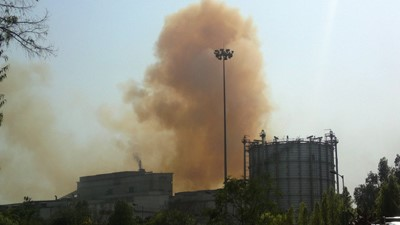
\includegraphics[width=80mm]{air.jpg}
 \caption{Air Pollution \cite{2}}
   \label{fig:Air Pollution}
\end{center}
\end{figure}

\subsection{Water Pollution}
It is the contamination of water bodies (e.g. lakes, rivers, oceans, aquifers and groundwater). It is caused by the discharge of waste water from commercial and industrial processes (intentionally or through spills) into water bodies; discharges of untreated domestic sewage, and chemical contaminants, such as chlorine, from sewage treatment plants; release of waste and contaminants into surface run-off flowing to surface waters (including urban run-off and agricultural run-off, which may contain chemical fertilizers and pesticides); waste disposal and leaching into groundwater; eutrophication and littering.

\begin{figure}[h]
 \centering
  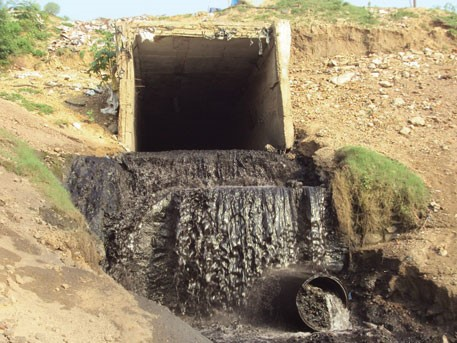
\includegraphics[width=50mm]{water.jpg}
  \caption{Water Pollution: Tata Steel discharge \cite{3}}
  \label{fig:Water Pollution: Tata Steel discharge}
\end{figure}

\subsection{Soil Pollution}
It is a part of land degradation is caused by the presence of XenoBionis (human-made) chemicals or other alteration in the natural soil environment. It is typically caused by industrial activity, agricultural chemicals, or improper disposal of waste, spill or underground leakage. Among the most significant soil contaminants are hydrocarbons, heavy metals, MTBE, herbicides, pesticides and chlorinated hydrocarbons.


\begin{figure}[h]
\centering
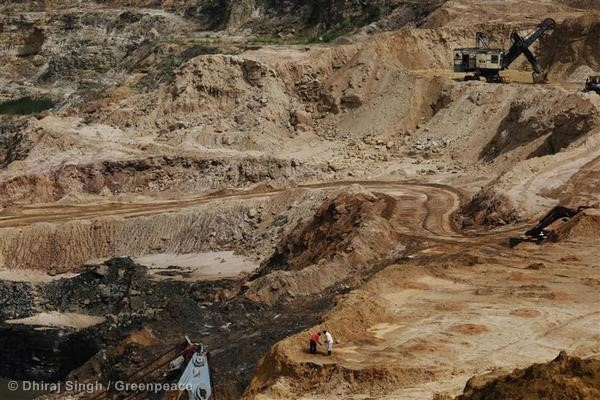
\includegraphics[width=0.4\textwidth]{./soil}\\[0.1in]
\label{Soil pollution: Durgapur coalmine}
 \caption{Soil Pollution Durgapur Coalmine \cite{4}}
 \label{soil pollution}
\end{figure}



\subsection{Noise Pollution}
Also known as noise disturbance is the disturbing or excessive noise that may harm the activity or balance of human or animal life. The source of most outdoor noise worldwide is mainly caused by machines and transportation systems, motor vehicles engines, aircraft, and trains.

%\begin{center}
%\begin{figure}
%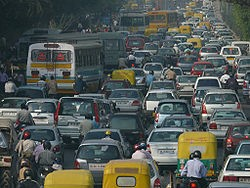
\includegraphics[width=0.6\textwidth]{./noise1}\\[0.1in]
 %\caption{noise pollution}
%\end{figure}
%\end{center}

\begin{figure}[h]
\centering
  
\includegraphics[width=70mm]{noise_pollution.jpg}
  \caption{Noise Pollution \cite{5}}
  \label{fig:Noise Pollution}
\end{figure}


\subsection{Radioactive Contamination}
It is resulting from 20th century activities in atomic physics, such as nuclear power generation and nuclear weapons research, manufacture and deployment. It is the deposition of, or presence of radioactive substances on surfaces or within solids, liquids or gases (including the human body), where their presence is unintended or undesirable. Such contamination presents a hazard because of the radioactive decay of the contaminants, which emit harmful ionising radiation such as alpha particles or beta particles, gamma rays or neutrons. The degree of hazard is determined by the concentration of the contaminants, the energy of the radiation being emitted, the type of radiation, and the proximity of the contamination to organs of the body.
%%\begin{center}
%\begin{figure}[h]
%\centering
%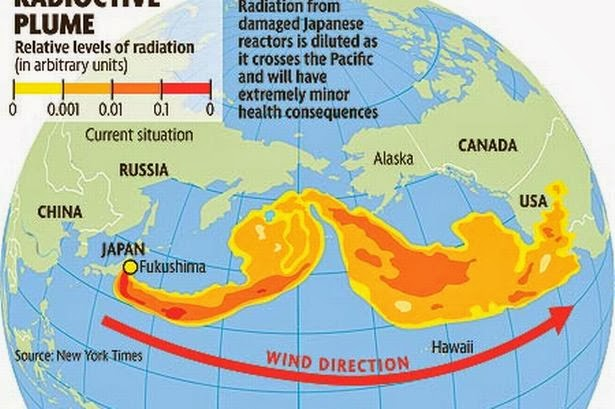
\includegraphics[width=0.00\textwidth]{./radiation}\\[0.1in] 
% %\caption{radioactive contamination}
%\end{figure}
%%\end{center}
%
%%\begin{figure}[h]
%%\centering
% % 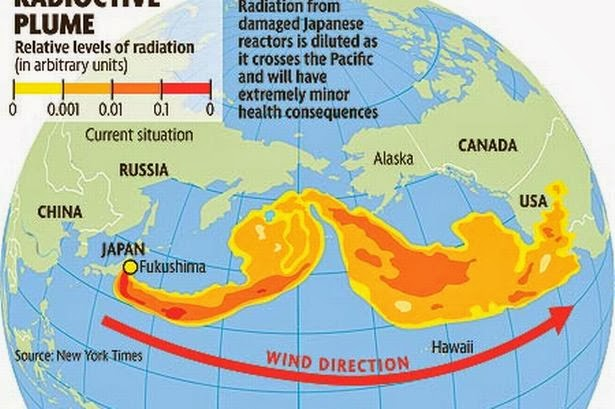
\includegraphics[width=70mm]{radiation.jpg}
%  %\caption{Radioactive Pollution \cite{6}}
%  %\label{fig:Radioactive Pollution}
%%\end{figure}




%%\subsection{Littering}
%%It consists of waste products that have been disposed improperly, without consent, at an inappropriate location.
%%\begin{figure}[h]
%%  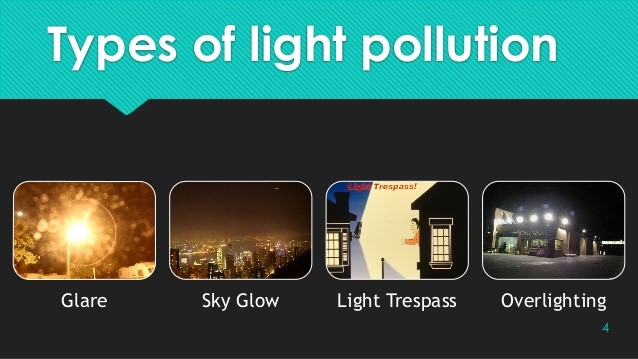
\includegraphics[width=\linewidth]{light_pollution.jpg}
%%  \caption{Air Pollution}
%%  \label{fig:Air Pollution}
%%\end{figure}

%\subsection{Thermal Pollution}
%It is the degradation of water quality by any process that changes ambient water temperature. A common cause of thermal pollution is the use of water as a coolant by power plants and industrial manufacturers. When water used as a coolant is returned to the natural environment at a higher temperature, the change in temperature decreases oxygen supply and affects ecosystem composition. Fish and other organisms adapted to particular temperature range can be killed by an abrupt change in water temperature (either a rapid increase or decrease) known as "thermal shock". Urban runoff—stormwater discharged to surface waters from roads and parking lots—can also be a source of elevated water temperatures.

%\begin{center}
%\begin{figure}
%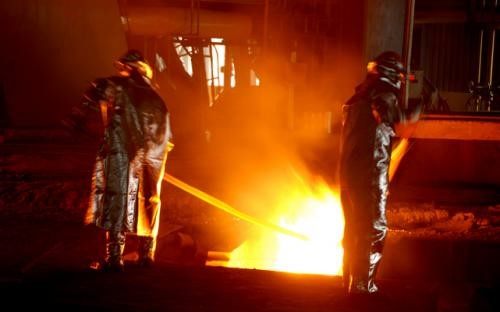
\includegraphics[width=0.60\textwidth]{./thermal}\\[0.1in]
 %\caption{Thermal pollution: SAIL Durgapur}
 %\label{Thermal pollution: SAIL Durgapur}
%\end{figure}
%\end{center}

%\begin{figure}[h]
 %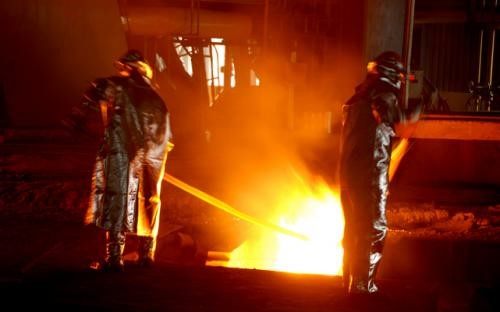
\includegraphics[width=\linewidth]{thermal.jpg}
  %\caption{thermal Pollution}
  %\label{fig:thermal Pollution}
%\end{figure}

%\subsection{Visual Pollution}
%It is an aesthetic issue and refers to the impacts of pollution that impair one's ability to enjoy a %vista or view. It disturbs the visual areas of people by creating harmful changes in the natural %environment. Pollution which can refer to the presence of overhead power lines, motorway billboards, %scarred landforms (as from strip mining), open storage of trash, municipal solid waste or space debris.

%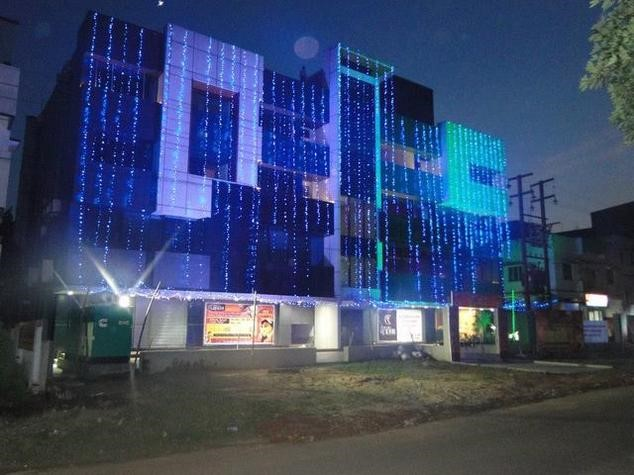
\includegraphics[width=1.0\textwidth]{./light}\\[0.1in]
%\begin{figure}[h]
 % 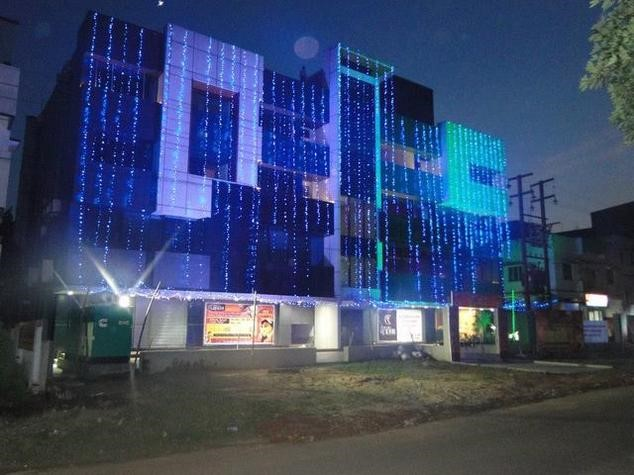
\includegraphics[width=\linewidth]{light.jpg}
  %\caption{light Pollution}
  %\label{fig:light Pollution}
%\end{figure}

%\subsection{Plastic Pollution}
%It involves the accumulation of plastic products in the environment that adversely affects wildlife, wildlife habitat, or humans. Plastics that act as pollutants are categorized into micro-, meso-, or macro debris, based on size.
%\begin{center}
%\begin{figure}
%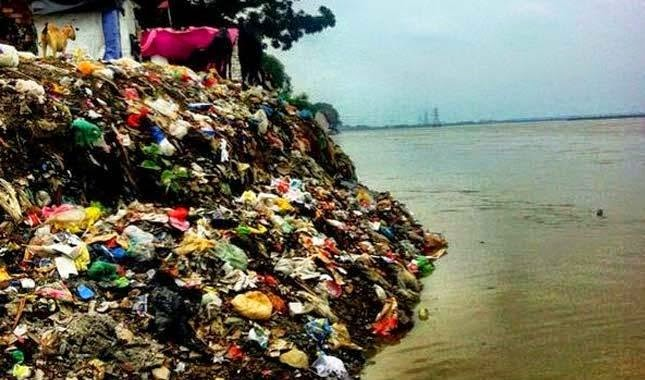
\includegraphics[width=0.70\textwidth]{./plastic}\\[0.1in]
 %\caption{Plastic Pollution}
%\end{figure}
%\end{center}

%\begin{figure}[h]
%\centering
 % 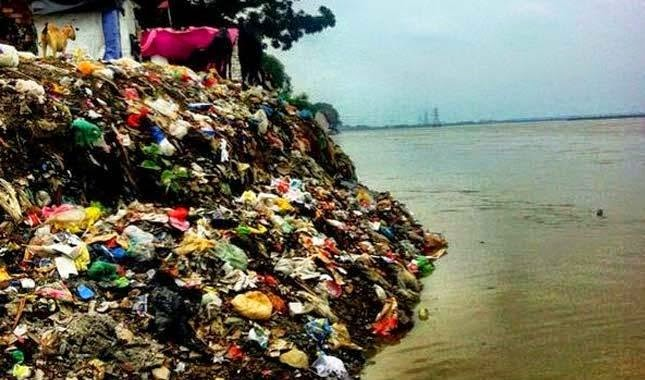
\includegraphics[width=100 mm]{plastic.jpg}
  %\caption{Plastic Pollution}
  %\label{fig:Plastic Pollution}
%\end{figure}

\section{Air Pollution}
Air pollution is by far the most harmful form of pollution in these times. Air pollution is caused by the harmful gases emitted by cars, buses, trucks, trains, and factories. Gases like sulphur dioxide $(SO_2)$, carbon monoxide(CO) and nitrogen dioxide ($NO_2$) are very harmful to the environment causing a lot of damage to humans, animals and the atmosphere. Evidence of increasing air pollution can be anticipated by the galloping rates of lung cancer, asthma, allergies, and various breathing problems along with severe and irreparable damage to flora and fauna. Even the most natural phenomenon of migratory bird has been hampered due to the contaminated air around the world.

\subsection{Air Pollutants}
An air pollutant is a substance suspended in the air that have adverse effects on humans, animals and the ecosystem. The substance can be solid particles, liquid droplets, or gases. A pollutant can be of natural origin or artificially produced. Pollutants are classified as primary or secondary. Primary pollutants are usually produced from a process, such as ash from a volcanic eruption, carbon monoxide gas from motor vehicle exhaust, or the sulphur dioxide released from factories. Secondary pollutants are not emitted directly. Rather, they form in the air when primary pollutants react or interact with other elements or compound in nature. Ground level ozone is a prominent example of a secondary pollutant. Some pollutants may be both primary and secondary: they are both emitted directly and formed from other primary pollutants.
\\
\\
Substances emitted into the atmosphere by human activity includes:
\subsubsection{(A) Nitrogen Dioxide}
\textbf{Nature and Sources of the Pollutant}: Nitrogen dioxide belongs to a family of highly reactive gas called Nitrogen Oxides ($NO_x$). These gases are formed when fuel is burned at high temperatures, and come principally from motor vehicle exhaust and stationary sources such as electric utilities and industrial boilers.
\\
\\
\textbf{Health and Other effects}: Nitrogen dioxide can irritate the lungs and lower resistance to the respiratory system of the human body causing infection such as influenza.
\\
\\
\textbf{Ambient Level}: EPA's health-based national air quality standard for $NO_2$ is 0.053 ppm

\subsubsection{(B) Sulphur Dioxide}
\textbf{Nature and Sources of the Pollutant}: Sulphur dioxide belongs to the family of Sulphur dioxide gases ($SO_x$). These gases are formed when fuel containing Sulphur (mainly coal and oil) is burned, and during metal smelting and also in many other industrial processes.
\\
\\
\textbf{Health and Other Effects}: The major health concerns associated with exposure to high concentrations of $SO_2$ include effects on breathing, respiratory illness, alterations in pulmonary defences, and aggravation of existing cardiovascular disease. Together, $SO_X$ and $NO_X$ are the major precursors to acid rain, which is associated with the acidification of fresh water lakes and streams, accelerated corrosion of buildings and monuments, and reduced visibility. 
\\
\\
\textbf{Ambient Level}: EPA's health-based national air quality standard for $SO_2$ is 0.03 ppm (measured on an annual average) and 0.14 ppm (measured over 24 hours).

\subsubsection{(C) Carbon Monoxide}
\textbf{Nature and Sources of the Pollutant}: Carbon monoxide is a colourless and odourless poisonous gas formed when carbon in fuels is not burned completely. It is a by-product of motor vehicle exhaust, which contributes more than two-thirds of all CO emissions nationwide.
\\
\\
\textbf{Health and Other Effects}: Carbon monoxide enters the bloodstream and reduces oxygen delivery to the body's organs and tissues. The health threat from CO is most serious for those who suffer from cardiovascular disease. Elevated CO levels is associated with visual impairment, reduced work capacity, reduced manual dexterity, poor learning ability, and difficulty [measured over 8 hours] in performing complex task.
\\
\\
\textbf{Ambient Level}: EPA's health based national air quality standard for CO is 9 parts per million (PPM).

\subsubsection{(D) Carbon Dioxide}
Because of the role of Carbon Dioxide ($CO_2$) as a greenhouse gas it has been described as "the leading pollutant" and "the worst climate pollution". Against this, it is argued that carbon dioxide ($CO_2$) is a natural component of the atmosphere, essential for plant life and respired out by the human and animal respiratory system. This question of terminology has practical effects, for example as determining whether the U.S. Clean Air Act is deemed to regulate $CO_2$ emissions. $CO_2$ currently forms about 405 parts per million (ppm) of earth's atmosphere, compared to about 280 ppm in pre-industrial times, and billions of metric tons of $CO_2$ are emitted annually by burning of fossil fuels. $CO_2$ increase in earth's atmosphere has been accelerating.

\subsubsection{(E) Particulate matter ($PM_{1O}$, $PM_{2.5}$ and $PM_1$)}
\textbf{Nature and Sources of the Pollutants}: Particulate matter is the term for solid or liquid particles found in the air. They originate from a variety of mobile and stationary sources (diesel trucks, wood stoves, power plants etc.).
\\
\\
\textbf{Health and Other Effects}: Major concerns for human health from exposure to particulate matter are- effects on breathing and respiratory systems, damage to lung tissue, cancer, and premature death.
\\
\\ 
\textbf{Ambient Level}: EPA's health-based national air quality standard for $PM_{10}$ is 50  $\mu$g /$m^3$ (measured as an annual average).

\subsection{Types of Air Pollution}
\textbf{Outdoor Air Pollution}:
Smog is a type of large-scale outdoor pollution. It is caused by chemical reactions between pollutants derived from different sources, primarily automobile exhaust and industrial emissions. Cities are often centres of these types of activities, and many suffer from the effects of smog, especially during the warm months of the year.
\\
\\
\textbf{Indoor Air Pollution}:
Indoor air pollution is the presence of one or more contaminants indoors that carry a certain degree of human health risk. Indoor air issues may be traced to the beginning of civilization. Prehistoric records note the problem of smoke in caves. However, over the last three decades the public has become more aware of indoor air pollution. Various studies show that people spend 65 to 90 percent of their time indoors; 65 percent of that time is spent at home. Field studies of human exposure to air pollutants indicate that indoor air levels of many pollutants may be two to five times, and on occasion more than one hundred times, higher than outdoor levels.

\subsection{Effects of Air Pollution}
Air pollution can affect our health in many ways with both short-term and long-term effects. Different groups of individuals are affected by air pollution in different ways. Some individuals are much more sensitive to pollutants than are others. Young children and elderly people often suffer more from the effects of air pollution. People with health problems such as asthma, heart and lung disease may also suffer more when the air is polluted. The extent to which an individual is harmed by air pollution usually depends on the total exposure to the damaging chemicals, i.e., the duration of exposure and the concentration of the chemicals must be taken into account.
\\
\\
Examples of short-term effects include irritation to the eyes, nose and throat, and upper respiratory infections such as bronchitis and pneumonia. Other symptoms can include headaches, nausea, and allergic reactions. Short-term air pollution can aggravate the medical conditions of individuals with asthma and emphysema. In the great “Smog Disaster” in London in 1952, four thousand people died in a few days due to the high concentrations of pollution.
\\
\\
Long-term health effects can include chronic respiratory disease, lung cancer, heart disease, and even damage to the brain, nerves, liver, or kidneys. Continual exposure to air pollution affects the lungs of growing children and may aggravate or complicate medical conditions in the elderly. It is estimated that half a million people die prematurely every year in the United States as a result of smoking cigarettes.


\subsection{Increasing Mortality Rate due to Air Pollution}
 The World Health Organization estimated in 2014 that every year air pollution causes the premature death of some 7 million people worldwide. India has the highest death rate due to air pollution. India also has more deaths from asthma than any other nation according to the World Health Organization. In December 2013 air pollution was estimated to kill 500,000 people in China each year. There is a positive correlation between pneumonia-related deaths and air pollution from motor vehicle emissions.
\\
\\
Annual premature European deaths caused by air pollution are estimated at 430,000. An important cause of these deaths is nitrogen dioxide and other nitrogen oxides ($NO_x$) emitted by road vehicles. Across the European Union, air pollution is estimated to reduce life expectancy by almost nine months. Causes of deaths include strokes, heart disease, COPD, lung cancer, and lung infections.
\\
\\
Urban outdoor air pollution is estimated to cause 1.3 million deaths worldwide per year. Children are particularly at risk due to the immaturity of their respiratory organ systems.\cite{7}
\begin{figure}[h]
\centering
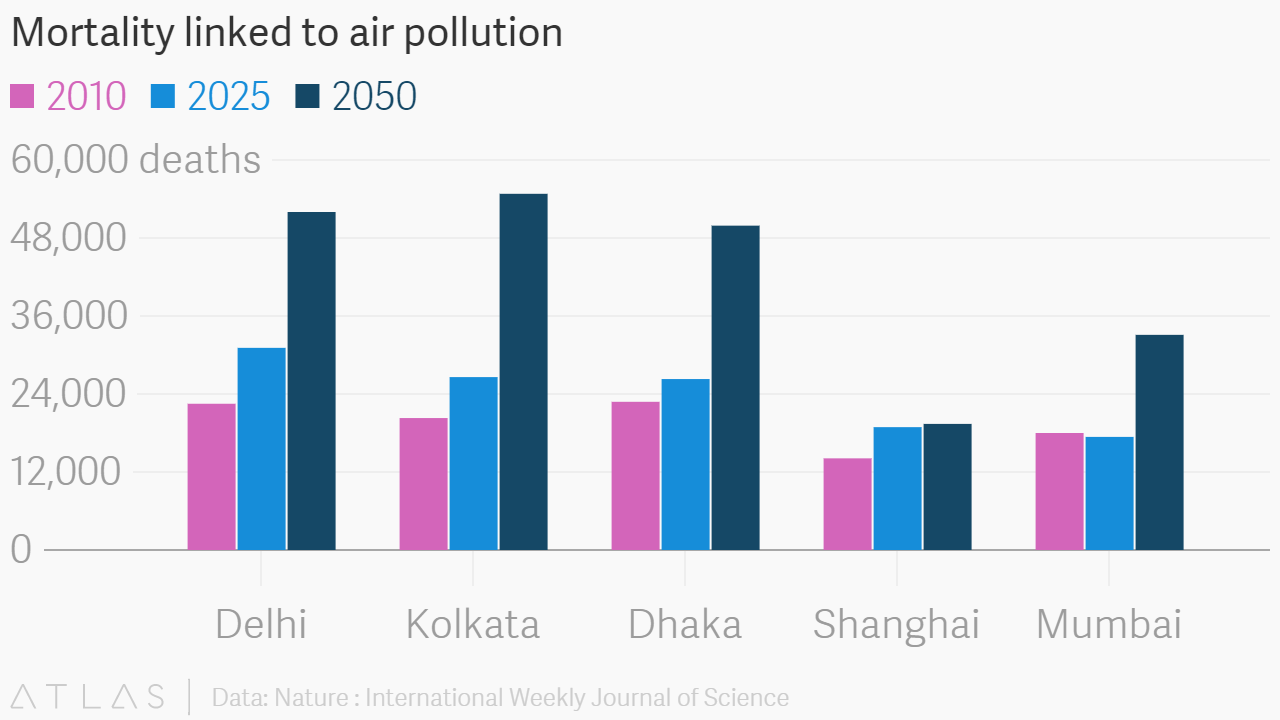
\includegraphics[width=0.8\textwidth]{./deadly}\\[0.1in]
\caption{Mortality linked to Air Pollution \cite{8}}
\label{fig: Mortality Linked to Air Pollution}
\end{figure}


\subsection{Major Air Pollution Incidents}

\subsubsection{Bhopal Gas Leak}
The world’s worst ever industrial accident happened on the night of December 2-3, 1984, when toxic gases leaked from the Union Carbide (now Dow Chemical) pesticide plant in Bhopal, India. The deadly fumes drifted into the sleeping city and people woke with burning eyes and lungs.
\\
\\
Thousands died within days. In the years after, pollutants seeping out of the plant site into groundwater have caused cancer, growth retardation and dizziness, say residents in Bhopal.\cite{9}

\subsubsection{Chernobyl Nuclear Accident}
The biggest radiation contamination ever happened on April 26, 1986 when the Chernobyl nuclear power plant’s core went into meltdown, killing 30 people and releasing 100 times more radiation than the atom bombs dropped on Japan. Even more radioactivity remains trapped within the plant.
\\
\\
From 1992 to 2002 in Belarus, Russia and Ukraine more than 4000 cases of thyroid cancer were diagnosed among children and adolescents, mainly due to contaminated milk. The 19-mile exclusion zone around the plant remains uninhabitable.\cite{9}

\subsubsection{Gulf of Mexico Oil and Gas Spill}
On April 20, 2010 the Deepwater Horizon offshore oil rig in the Gulf of Mexico exploded, killing 11 workers and leading to the worst oil spill and environmental catastrophe in US history.
\\
\\
A ruptured underwater pipe spewed almost 5 million barrels of oil into the Gulf over three months, threatening hundreds of miles of beaches, wetlands, and estuaries. Thousands of animals, including turtles, crabs, fish, and birds fell victim, and the local fishing and tourism industries suffered badly.\cite{9}
\begin{figure}[h]
\centering
  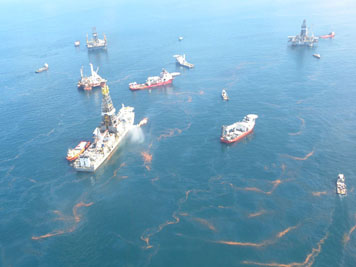
\includegraphics[width=60mm]{dwh-oil-spill-view-over-rig.jpg}
  \caption{Oil and Gas spill in Gulf of Maxico \cite{28}}
  \label{fig:Noise Pollution}
\end{figure}

\subsection{Air Quality Index}
Air quality index (AQI) is a number used by government agencies  to communicate to the public how polluted the air currently is or how polluted it is forecast to become. As the AQI increases, an increasingly large percentage of the population is likely to experience increasingly severe adverse health effects. Different countries have their own air quality indices, corresponding to different national air quality standards.

\begin{figure}[h]
\centering
  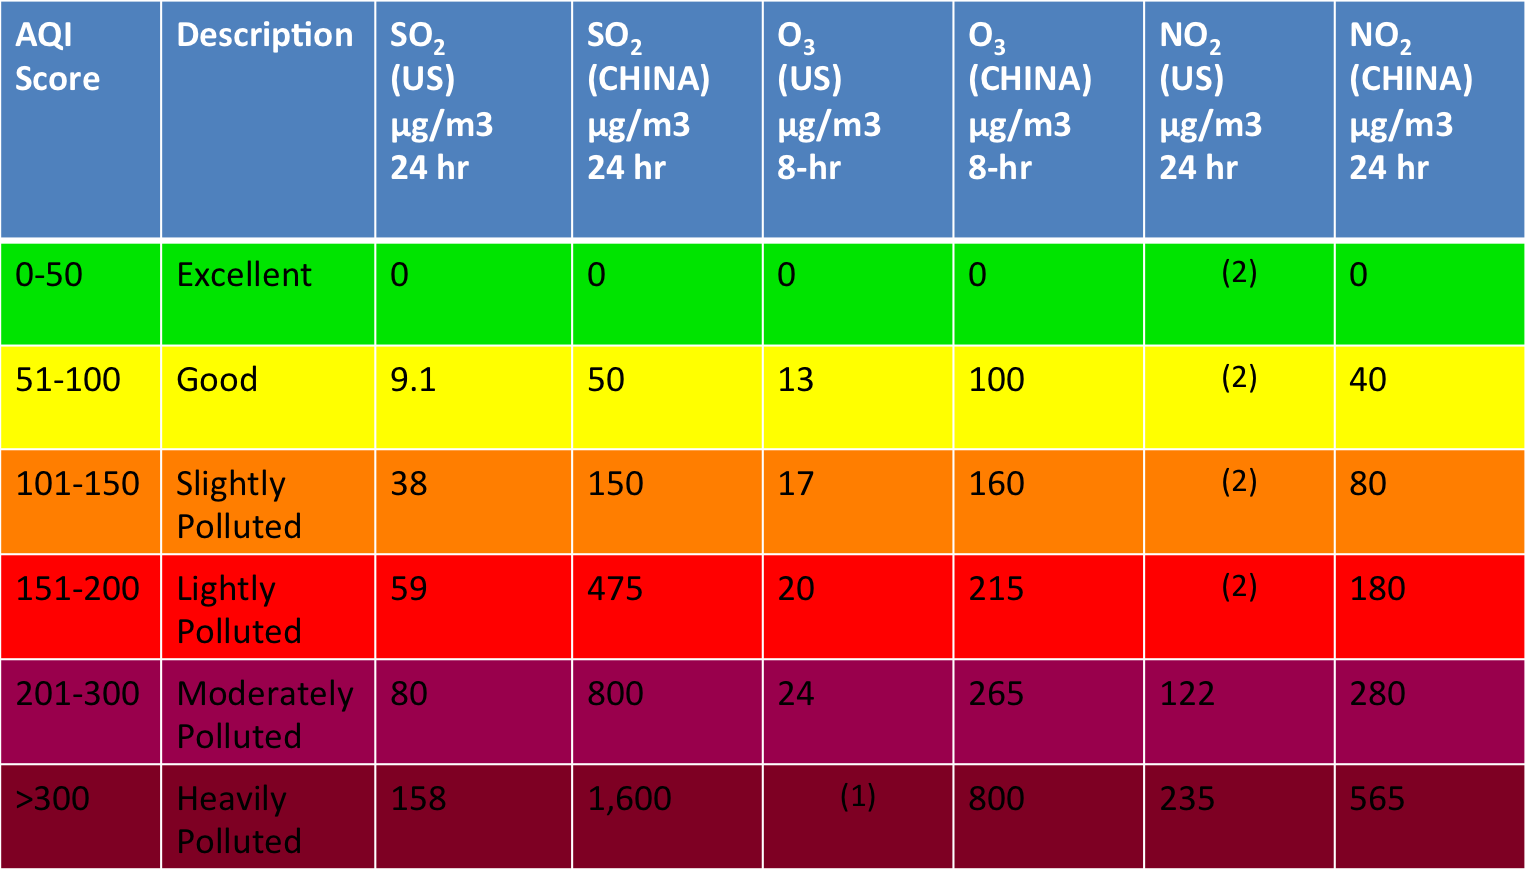
\includegraphics[width=0.8\textwidth]{./AQI}\\[0.1in]
  \caption{AQI categories and breakpoint concentrations with averaging times \cite{10}}
  \label{fig:AQI Category Breakpoint}
\end{figure}


The concept of an air quality Index (AQI) that transforms weighted values of individual air pollution related parameters (e.g. $SO_2$, CO, visibility, etc.) into a single number or set of numbers is widely used for air quality communication and decision making in many countries. Thus, An AQI is defined as an overall scheme that transforms weighted values of individual air pollution related parameters ($SO_2$. CO, visibility, etc.) into a single number or set of numbers.
%\begin{figure}[h]
 % 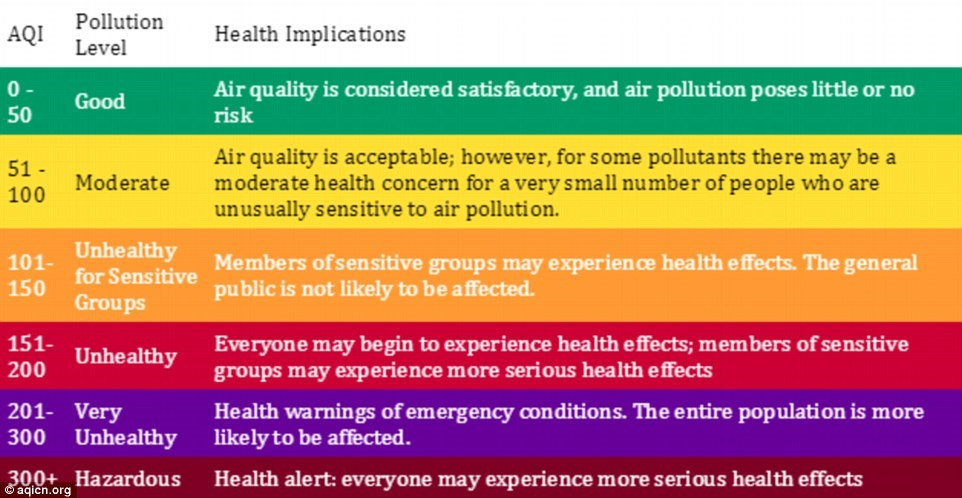
\includegraphics[width=\linewidth]{aqi2.jpg}
  %\caption{AQI levels}
  %\label{fig:AQI levels}
%\end{figure}

\section{Comparison of Indoor and Outdoor air pollution}
We have done a comparison on Indoor and Outdoor Pollution basically on its impact Biotic and Abiotic Component.

\subsection{Why is indoor air pollution more hazardous than outdoor air pollution?}

According to the EPA, our indoor environment is two to five times more toxic than our outdoor environment, and in some cases, the air measurements indoors have been found to be 100 times more polluted.
\\
\\
The International Agency for Research on Cancer and the World Health Organization have concluded that 80\% of all cancers are attributed to environmental rather than genetic factors, including exposure to carcinogenic chemicals, many of which are found in household cleaning products.
\\
\\
The World Health Organization (WHO) agrees, reporting that almost 3\% of the global burden of disease is due to indoor air pollution. We spend as much as 90\% of our lives indoors nowadays and researchers are investigating our exposure to indoor pollutants as contributing causes to rising incidence of autism, allergies and toxin load.
\\
\\
\subsection{Why do we need to measure air pollution?}

According to a report published earlier this year by the World Health Organisation, air pollution now kills approximately seven million people annually, worldwide. This accounts for as much as one in eight deaths, and is by far the single biggest environmental health risk.
\\
\\
In order to counteract this alarming statistic and take action to clean up air , it’s important to first understand where the pollution is most concentrated, how it occurs, what elements are involved and how we can neutralise them. In order to do this, comprehensive air monitoring must be undertaken on a national and international scale.
\\
\\
Among other pollutants, air monitors assess the amounts of carbon dioxide ($CO_2$), carbon monoxide (CO), nitrogen oxides ($NO_x$), ozone ($O_3$) and particulate matter 2.5 ($PM_{2.5}$). This allows us to see where and why pollution occurs, so that we can not only actively avoid overly contaminated areas in our daily routines but also try to implement measures to curb such pollution.

\begin{figure}[h]
\centering
  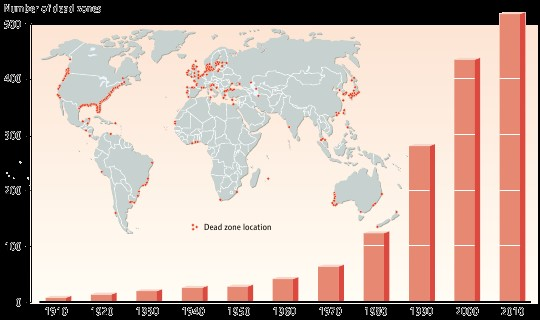
\includegraphics[width=80mm]{deadzone.jpg}
  \caption{AQI levels}
  \label{fig:AQI levels}
\end{figure}


\section{Site Survey}

\subsection{Present Scenario of Air Pollution}
Greenpeace analysed NASAs satellite data on particulate matter from 2003 to 2015 in India and China, and found that pollution levels in Chino peaked in 2011 and then started to gradually reduce. India, however, saw a spike over the past decade, the last year being the worst on record. The study looked at the aerosol optical depth (A0D), which is h the amount of fine solid particles and liquid droplets in air. The levels in India have increased over the years with north India being the most polluted part of the country. The biggest jump was seen in West Bengal, Bihar, Uttar Pradesh and the National capital Region. The report said that the AOD levels in Indian cities Patna, Kolkata, Delhi, Gorakhpur, Kanpur and Varanasi all went up from 2005 to 2015.
\\
\\
There are large numbers of industries within West Bengal which are emitting harmful gases into the atmosphere and as a matter of fact, this emission is leading to tremendous amount of air pollution in major cities like Kolkata, Asansol, Durgapur and Raniganj. The extent of this pollution is so high, as to raise some serious environmental concerns. Presence of a large number of industries in Durgapur is the single biggest reason for the high level of pollution in this industrial industrial town and the biggest hurdle in the growth of this steel city and the only fact of concern for a healthy living.\cite{11}

\begin{figure}[h]
\centering
  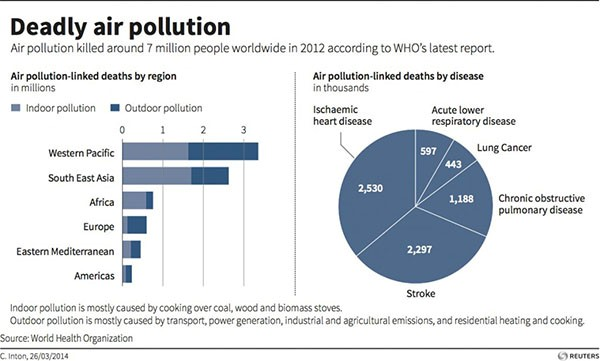
\includegraphics[width=90mm]{site_survey1.jpg}
  \caption{AQI levels \cite{12}}
  \label{fig:AQI levels}
\end{figure}

\begin{figure}[h]
\centering
  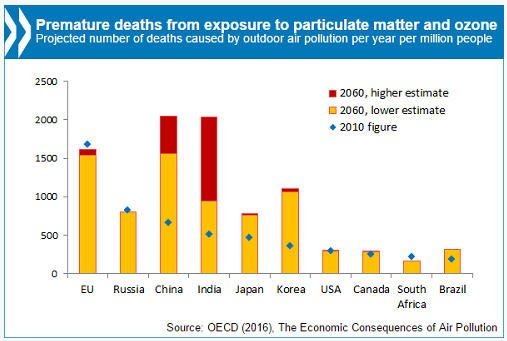
\includegraphics[width=90mm]{site_survey2.jpg}
  \caption{AQI levels \cite{13}}
  \label{fig:AQI levels}
\end{figure}

\subsection{Status of Air Pollution in Durgapur}
With pollution level increasing dangerously in the industrial belts of Haldia and Asansol, the union ministry of environment and forest had imposed a ban in 2010 declaring that no further industries could be set up in these industrial belts, the areas were classified as critically polluted zones. The centre as shortlisted Durgapur as the stage 2 of the smart city mission and the local civic body arranged a public hearing in this connection. The Durgapur Projects Limited (DPL), a state owned power utility, was asked to suspend generation as it continues to release Suspended Particulate Matter (SPM) in the ambient air. In December 2002 the WBPCB had introduced states first ambient air quality monitoring station in Durgapur, which however failed after a couple of years.
\\
\\
\textbf{NEWS FEED:}
\cite{14}
\\
\\
\begin{enumerate}
	\item On 12th June 2015 Durgapur steel plant was hit by another mishap.
	\item On August 24, the West Bengal Pollution control board registered a police complaint against Durgapur Projects Limited (DPL), a state government undertaking, for violating pollution norms.
	\item Durgapur News Services, 26 December 2014: Recent revelation of the fact that pollution linked cancer patients on rise in Asansol-Durgapur.
\end{enumerate}

\subsection{Major Industries and pollutants emitted by them}

\begin{center}
 \begin{tabular}{| c |  p{4cm} | p{4cm} | p{4cm}| } 
 \hline
 Sl. & NAME & PRODUCT & POLLUTANTS \\ [0.5ex] 
 \hline\hline
 1 & Durgapur Steel Plant (D.S.P.) & P.R. TNIT Bars \& Rods, Angles, Channels, Wheel \& Axle & $S0_2$, $NO_x$, $CO_3$, Pb, Ni, As, Cd, Cr, ZnSe, Hg, PM \\ 
 \hline
 2 & Durgapur Thermal Power Station(D.V.C.) & P.R. Power Generation & $S0_2$, $NO_x$, Ni, As, Cr, Hg, Acid gases $S0_2$, $NO_x$, Hg, Acid gases \\
 \hline
 3 & The Durgapur Projects Ltd(D.P.L.)  & P.R. Power, Coke, Industrial Gas, Domestic Power, Industrial Power & $S0_2$, $NO_x$, Ni, As, Cr, Hg, Acid gases \\
 \hline
 4 & NTPC-SAIL Power CO Ltd & P.R. Power Generation \& Distribution & $S0_2$, $NO_x$, Ni, As, Cr, Hg, Acid gases \\
 \hline
 5 & Alloy Steel Plant & P.R. Stainless Steel, Billets etc. & Smoke, Fume, CO, Organic 
gases, PM, Organic matter \\
 \hline
 6 & Bharat Petroleum Corp. Ltd  & P.R. Petroleum Products \& Lubricants & $CO_2$, CO, methanol, soot, benzene, acid rains \\
 \hline
 7 & Birla Corporation Ltd  & P.R. Portland Slag Cement & $S0_2$, $NO_x$, CO, $CO_2$ \\
\hline
 8 & Durgapur Cements Works  & Cements Works & $S0_2$, $NO_x$, CO, $CO_2$ \\ 
\hline
 9 & Durgapur Chemicals Ltd.  & P.R. Caustic Soda, Benzene, Bleaching Powder, Sodium Chlorophenate, Hydrogen Gas, etc. & $S0_2$, $NO_x$, Benzene, Organic gases, Cl etc. \\
\hline
 10 & Graphite India Ltd  &Products of Graphite & PM, hydrocarbons, organic matter etc. \\  [1ex] 
 \hline
\end{tabular}
\end{center} %objective changed to problem definition
\chapter{LITERATURE SURVEY} % Main chapter title

\label{Chapter2} % For referencing the chapter elsewhere, use \ref{Chapter1} 


\section{Air Quality Monitoring }

Environment monitoring is crucial and necessary task in enabling healthy living of mankind. Environment monitoring is critical to know whether the quality of our environment is getting better or worse. Information gathered through environment monitoring is important to many decision makers, inside and outside the government. With the results of monitoring, the government can make informed decision about how the environment will affect people and how people are affecting the environment. A lot more work has been done in the area of air quality monitoring system in past years which is summarised below: -

\subsection{Indoor Air Quality Monitoring}
In recent years, indoor air quality (IAQ) has drawn considerable attention in both the public and scientific domains, due to the fact that most buildings appear to fall far short of reasonable air quality goals. Statistics from the U.S. Environmental Protection Agency(EPA) indicate that, on average, the indoor levels of pollutants are two to five times higher than outdoor levels and people in the U.S. spend about 90\% of their time indoors. Bad indoor air quality influences human health, safety, productivity, and comfort. IAQ is important and different people have different exposure to pollutants. Providing personalized IAQ information has the potential to increase public awareness of the relationship between their behaviour and air quality; help people to improve their living environments; and also provide valuable information to building managers, policy makers, health professionals, and scientific researchers.
\\
\\
Indoor air quality monitoring is necessary as sometimes we find that indoor level of pollution is higher than outdoor pollution level. This is because of low ventilation and cooking and heating processes. Some of the Indoor Pollution work has been surveyed and their gist is given below.

\subsubsection{Pollution Monitoring System using Wireless Sensor Network \cite{15} }
In this paper they simulated the three air pollutants gases including carbon monoxide, carbon dioxide sulphur dioxide in air. They also apply the approach in various applications like leaking cooking gas in our homes, to alert the workers in oil gas industry to detect the leakage etc. In this they used a sensing unit, a processing unit in the microcontroller, a radio component. The node is designed by integrating the sensor associate circuitry, Atmega 328p low power microcontroller and Xbee communication module. The operating system that runs in the Xbee, coordinates the substances measurement process the acquisition of the change in gas percentages in air and coordinates with the Xbee module for data transmission to the zigbee router. The pollution detector consists array of sensors. 
 Dependence Power consumption of sensor nodes need to be minimized. The selection of sensor and material used in construction of the sensor should select such that there should be minimum changes in the accuracy of the system. In May 2012 V. Ramya and B. Palaniappan worked on the topic Embedded system for Hazardous Gas detection and Alerting by designing a microcontroller based toxic gas detecting and alerting system which sensed gases like LPG and propane and displayed on LCD. Also an alarm was generated and SMS alert were sent to authorized person through the GSM when the level of gases exceeds certain limit.
The system was designed using PIC 16F877 Microcontroller and sensors MQ-2 and MQ-7 for sensing LPG and Propane respectively and displayed on the monitor. When the level of LPG and Propane exceeds a critical level (LPG 1000 ppm and Propane 10000ppm), then an alarm is generated and SMS is sent to the authorized user. But here only two gases are detected (LPG and Propane) but lacks the detection of other harmful pollutant which are present in the environment. Although it is an automated system but it requires to reset after every critical situations.

\subsubsection{Indoor Air Quality in Homes, Offices \& Resturants in Korean Urban Areas—Indoor Outdoor Relationship \cite{16}}
In this paper, Indoor air quality was monitored and measured pollutants were respirable suspended particulate matter (RSP), carbon monoxide (CO), carbon dioxide ($CO_2$), nitrogen dioxide ($NO_2$), and a range of volatile organic compounds (VOCs). In addition, in order to evaluate the effect of smoking on indoor air quality, analyses of parameters associated with environmental tobacco smoke (ETS) were undertaken, which are nicotine, ultraviolet (UVPM), florescence (FPM) and solanesol particulate matter (SolPM). Further both indoor and outdoor air quality were measured and compared and Impact of seasonal differences on both indoor and outdoor air quality were also studied. It was found that indoor pollution in winters was comparatively higher than summer. Indoor Air quality difference due to difference in location were studied and compared. Impact of outdoor pollution on indoor air quality were seen and examined.

\subsubsection{Investigation of Indoor Air Quality at Residential Homes in Hong Kong-case Study \cite{17}}
 Air pollutants measured in this study included carbon dioxide ($CO_2$), respirable suspended particulate matter ($PM_{10}$), formaldehyde (HCHO), volatile organic compounds (VOCs) and air borne bacteria. During the air measurement, indoor temperature, relative humidity and the age of the building were also recorded. A portable Q-Trak monitor (Model 8551, TSI Inc.) was used to monitor the indoor and outdoor $CO_2$ concentrations, temperature and relative humidity. The $CO_2$ analyser equipped with a thermistor and a thin film capacitive sensor is able to detect $CO_2$ based on the mechanism of non-disperse infrared detection. A Dust-Trak air monitor (Model 8520, TSI Inc.) was used to measure $PM_{10}$ concentrations.

\subsubsection{MAQS: A Personalized Mobile Sensing System for Indoor Air Quality Monitoring. \cite{18}}
This paper describes MAQS, a personalized mobile sensing system for IAQ monitoring.
To improve accuracy and energy efficiency, MAQS incorporates three novel techniques:
An accurate temporal n-gram augmented Bayesian room localization method that requires few Wi-Fi fingerprints.
An air exchange rate based IAQ sensing method, which measures general IAQ using only $CO_2$ sensors. 
A zone-based proximity detection method for collaborative sensing, which saves energy and enables data sharing among users.

\subsubsection{Detecting Indoor Air Pollutants and taking safety measures \cite{19}}
A sensor based e-nose is developed to sniff the pollutants presents in indoor environment by [1] to monitor indoor air quality (IAQ) and maintain good IAQ by controlling HVAC system of the room. Also the IAQ monitoring along with the relationship between health and IAQ is discussed but this lacks a proper architecture. The effect of outdoor air and indoor human activity on mass concentration of PM 10, PM 2.5, PM 1 is discussed. It is shown that concentration of carbon dioxide and $PM_{10}$ in domestic kitchen is greater than in living rooms showing that cooking is a major source of pollution. The influence of outdoor air quality on the indoor air quality is discussed. They also tried to provide quantitative information on the levels of potentially important pollutants in three typical environments (homes, offices, and restaurants), to compare indoor and ambient pollution as part of the task of source appointment, and investigate the extent to which certain indoor pollution sources influence the quality of indoor air in urban areas. The above study has confirmed the importance of ambient air quality in determining the quality of air indoors. Lower detection limits and precisions for the methods used in this study are the limitations of this work.

\subsection{Outdoor Air Quality Monitoring}
As there is increase in urbanisation leading to increased volume of traffic, market places, industries etc. the outdoor air quality is deteriorating day by day. Therefore there is a need of continuous air quality monitoring and using that information in the betterment of general public.

\subsubsection{Air Sensing and Alert Generation \cite{20}}
They simulated the three air pollutants gases including carbon monoxide, carbon dioxide and sulphur dioxide in air. They also apply the approach in various applications like leaking cooking gases in homes, to alert the workers in oil gas industry to detect the leakage etc. In this work they used a sensing unit, a processing unit in the microcontroller, a radio component. The node is designed by integrating the sensor associate circuitry, Atmega 328p low power microcontroller and Xbee, coordinates the substances measurement process the acquisition of the change in gas percentages in air and coordinates with the Xbee module for data transmission to the zigbee router. The pollution detector consist array of sensors. But Dependence Power consumption of sensor nodes need to be minimized and the selection of sensor and material used in construction of the sensor should be selected wisely. Similarly in a microcontroller based toxic gas detecting and alerting system was designing sensed gases like LPG and propane and displayed on LCD. Also an alarm was generated and SMS alert were sent to the authorized person through the GSM when the level of gases exceed certain limit. The system was designed using PIC 16F877 Microcontroller and sensors MQ-2 and MQ-7 for sensing LPG and Propane respectively and displayed on the monitor. When the level of the LPG and Propane exceeds a critical level (LPG greater than 1000 ppm and Propane greater than 10000 ppm), then an alarm is generated and SMS is sent to the authorized user. But here only two gases are detected and lacks the detection of other harmful pollutant which are present in the environment. Although it is an automated system but it requires to reset after every critical situation.

\subsubsection{Environment Monitoring and Air Quality Prediction \cite{21}}
We can use the Air Quality information along with some other useful information to predict the air quality depending upon different criteria. Different methods and modelling techniques can be used to predict air quality of any arbitrary location or time. Following are some literature survey using different useful technologies:-
Using a distance decay regression selection strategy
They reported the first attempt to model NO, $NO_2$ and $NO_x$ concentration in Los Angeles using a land use regression (LUR) approach. The LUR was developed as part of a study to examine the impacts of outdoor air pollution on respiratory health in children. The LUR method seeks to predict pollution concentrations at a given site based on surrounding land use, road network, traffic, physical environment and population characteristics using a series of buffers. In this work, NO, $NO_2$ and $NO_x$ concentrations for the LA metropolitan area were modelled using the ADDRESS modelling strategy. The final three prediction models explained 8186 Models. The model provides a relatively easy and feasible way to improve exposure analysis. The influence of slope gradients decreases suggesting that steeper gradient. It concludes that truck routes exerted higher $NO_x$ emissions and had a positive influence on concentration.
Using Machine Learning (semi-supervised learning) in Modelling and Predicting Air Quality
Machine learning and Artificial intelligence is widely used for prediction and classification purpose. Since Air quality depends upon many parameters in a non-linear way hence prediction work in regard to environmental monitoring needs to deal with large volume of data. Therefore, Neural Networks are best suited for this purpose. They use linear chain conditional random field (CRF) and Artificial neural network to infer the real-time and fine-grained air quality information throughout the city, based on the (historical and real-time) air quality data reported by existing monitor stations and a variety of data sources observed in the city, such as meteorology, traffic flow, human mobility, structure of road networks, and point of interests (POIs). It proposes a semi-supervised learning approach based on a co-training framework that consist of two separated classifiers. One is a spatial classifier based on Artificial Neural Network (ANN), which takes spatially-related features as input to model the spatial correlation between air qualities and different locations. The other is a temporal classifier based on a linear-chain conditional random field (CRF), involving temporally-related features to model the temporal dependency of air quality in a location.
The result show the advantage of this method over four categories of baselines, including linear/Gaussian interpolations, classical dispersion models, well-known classification models like decision tree and CRF, and ANN. The city was divided into disjointed grids assuming that air quality in a grid is uniform. Each has a geospatial coordinate and a set of AQI labels to be inferred or already associated if having an air quality monitor station located.

\subsubsection{Inferring Air Quality and location by using semi-supervised inference model Based on Urban Big Data Technology \cite{22}}
It is very complicated question to find out the most optimum location for placing the sensor to cover a large area and predict the air quality of whole area accurately. They tried two answer two questions in their work. First, to infer real-time air quality of any arbitrary location given environmental data and historical air quality data from very sparse monitoring locations. Second, if one needs to establish few new monitoring stations to improve the inference quality, and to determine the best locations for such purpose.
\\
\\
Here they designed a semi-supervised inference model utilizing existing monitoring data together with heterogeneous city dynamics, including meteorology, human mobility, structure of road networks and point of interests (POIs). It also proposes an entropy minimization model to suggest the best locations to establish new monitoring stations. Evaluation of the proposed approach using Beijing air quality data was done. They divided geo-spatial area into disjoint grids, which becomes the basic unit in inference. The AQI values of most grids were completely unknown while the historical AQI values of a small amount of grids can be obtained through existing monitoring stations.

\subsubsection{Mobile Environment Monitoring \cite{23}}
Small Environment Monitoring boxes dynamically moving around the city or given area can be much more efficient and feasible way to cover a large area for air quality monitoring. It can be much more effective method to gather data of more locations which in turn make the prediction process more realistic and accurate. Thus, designing an online GPRS Sensors Array for air pollution monitoring system can be done for this purpose. The system integrates a single chip micro controller, several air pollution sensors, a GPRS modem and a GPS module. The unit can be placed on the top of any moving device such as public transport vehicle. While the vehicle is on the move, the micro controller generates a frame consisting of the acquired air pollutant level from the sensors array and the physical location that is reported from the attached GPS module. The pollutants frame is then uploaded to the General Packet Radio Service Modem (GPRS-modem) and transmitted to the pollution-server for storing the pollutants level of further usage by interested clients such as production agencies, vehicles regeneration authorities, tourist and insurance companies. The pollution –server is interfaced to Google maps to display real-time pollutants levels and their locations. 
\\
\\
The system software architecture is divided into two layers structure i.e; physical layer and application layer. Physical layer is responsible for acquiring the real time data from the sensor-array and physical location, time and date of the sampled pollutants from the GPS module and is implemented using ANSI C language which is compiled to native microcontroller code. The application layer consist of three primary module: Socket-Server, Air Pollution Index and Google-Mapper. Socket-Server collects and stores data from all the mobile-DAQs. Air Pollution Index calculates pollution categories based on local pollution policies and regulations. But the limitation is that the data collected is limited to the vicinity of six monitoring stations. Also this system monitors only three pollutants that is CO, $NO_2$ and $SO_2$.

\subsubsection{Comparison of different approaches of Air Quality Prediction \cite{24}}
A comprehensive comparison between different prediction approaches gives us the idea to select best approach to proceed in a systematic way. In prediction of pollutants $PM_{10}$ and Ozone has been taken into consideration. Here feed forward neural networks (FFNNs), recognized as state-of-the-art approach for statistical prediction of air quality, and are compared with two alternative approaches derived from machine learning: pruned neural networks (PNNs) and lazy learning (LL). All the three approaches are tested in the prediction of ozone and $PM_{10}$ and the predictors are trained. The prediction, issued at 9 a.m. for the current day, show a satisfactory reliability. LL provides the best performances on indicators related to average goodness of the prediction, while PNNs are superior to the other approaches in detecting of the exceedances of alarm and attention thresholds. The better outcome of all the approaches on $PM_{10}$ with respect to ozone can be due to daily average prediction target, which generates a smoother time series than the maximum 8-h moving average adopted for ozone.

\subsubsection{A Mobile GPRS-Sensors Array for Air Pollution Monitoring \cite{25}}
Designing an online GPRS-Sensors Array for air pollution monitoring system can be done. The system integrates a single chip micro controller, several air pollution sensors, a GPRS modem and a GPS module. The unit can be placed on the top of any moving device such as a public transportation vehicle. While the vehicle is on the move, the micro controller generates a frame consisting of the acquired air pollutant level from the sensors array and the physical location that is reported from the attached GPS module. The pollutants frame is then uploaded to the General Packet Radio Service Modem (GPRS-Modem) and transmitted to the Pollution-Server via the public mobile network. A database server is attached to the Pollution-Server for storing the pollutants level for further usage by interested clients such as environment production agencies, vehicles regeneration authorities, tourist and insurance companies. The pollution-Server is interfaced to Google maps to display real-time pollutants levels and their locations. The system software architecture is divided into two layers structure i.e; physical layer and application layer. Physical layer is responsible for acquiring the real- time data from the sensors-array and the physical location, time and date of the sampled pollutants from the GPS module and is implemented using ANSI C language which is compiled to native microcontroller code. The application layer consists of three primary modules: Socket-Server, Air-Pollution-Index, and Google-Mapper. Socket-Server collects and stores pollutant data from all the Mobile-DAQs. Air Pollution-Index calculates pollution categories based on local pollution policies and regulations. Finally, Google-Mapper, makes this pollution information available over the Internet. But the limitations are that the data collected is limited to the vicinity of the six monitoring stations. Also this system monitors only three pollutants that is CO, $NO_2$ and $SO_2$.

\subsubsection{Inferring Air Quality Based on Urban Big Data \cite{26}} 
They tried to answer two questions in their work. First, to infer real-time air quality of any arbitrary location given environmental data and historical air quality data from very sparse monitoring locations. Second, if one needs to establish few new monitoring stations to improve the inference quality, how to determine the best locations for such purpose? Here they designed a semi-supervised inference model utilizing existing monitoring data together with heterogeneous city dynamics, including meteorology, human mobility, 5 structure of road networks, and point of interests (POIs). It also proposes an entropy minimization model to suggest the best locations to establish new monitoring stations. Evaluation of the proposed approach using Beijing air quality data was done. They divide geo-spatial area into disjointed grids, which be-comes the basic unit or instance in the inference. Each grid, denoted by r, is a 1km*1km sub-area, with its own geographical coordination. Each grid is associated with an AQI value, of which some need to be inferred. The AQI values of most grids were completely unknown while the historical AQI values of a small amount of grids can be obtained through existing monitoring stations. The meteorology, road network, and POI information of each grid are assumed to be available. The goal was to infer the AQI distribution of any unobserved location v at any given time stamp t(i). The proposed algorithm consists of four stages. In the first stage construction of a spatial-temporal graph, the AQI Affinity Graph (AG) was done to model the spatial-temporal correlation between grids. In the second stage they try to learn the weights of the edges, assuming they represent the correlations between nodes based on their features. The third stage emphasizes on inferring the AQI values for locations. In this stage model presumes those grids whose features were close to each other tend to share similar AQI values. In the final stage the feature weights are adjusted to minimize the uncertainty of the model on inferring the unobserved locations. Finally to recommend the most proper locations in which building new air-quality monitoring stations can lead to the largest accuracy improvement on air quality inference, they proposed entropy-minimization greedy technique which tries to identify a set of nodes that are uncorrelated with the more confident (i.e. low entropy) ones most of the time as the recommended locations for deployment. It is much more effective than myopically minimize entropy or other heuristics. Efficiency of this model could be increased through parallelization.
 %literature survey included in this
\chapter{System Architecure} % Main chapter title

\label{Chapter3} % For referencing the chapter elsewhere, use \ref{Chapter1} 

The Complete System Architecture has been divided into following modules: Sensing Module, Controlling and Processing Module, Communication Module and Power Module.

\section{Sensing Module}
A sensor is a electronic device that generates signals upon detecting/sensing any physical conditions or chemical compounds, it's designed to detect. It is also defined as any device that converts a signal from one form to another. These are built with mostly electrical or electronic components. Our Sensing Unit comprises of sensors measuring different air-pollutants present in the air such as Nitrogen Oxide, Sulphur Dioxide, Carbon Monoxide, Carbon dioxide, and Particulate Matter.

\subsection{Sensor Description}
We have made our environment monitoring box with both High Quality Gas sensors as well as Low quality Gas sensors. They are used to make the device more robust, portable, sensitive, reliable and at the time cheaper.

\subsubsection{Low Quality Sensor}
We started our work with Environment Monitoring Box with some low quality sensors which are readily available and are incapable of measuring pollutants accurately but approximately. They give an indication of increase in pollutant level. They have a longer heating time and are less sensitivity. We have used the following semiconductor type Gas sensors:
\\
\\
\begin{enumerate}
	\item Semiconductor type Gas sensor: These devices are made up of heated metal oxides which are used for measurement of gas concentration of a target gas by measuring the electrical resistance of the device.
	\begin{itemize}
		\item \textbf{MQ-135}: It is used in air quality monitoring equipments for buildings/offices , suitable for detecting of $NH_3$, $NO_x$, alcohol, benzene, smoke, $CO_2$, etc. This sensor is composed of micro $Al_2O_3$ ceramic tube, Tin Dioxide ($SnO_2$) sensing layer, measuring electrode and a heater which are fixed into a crust made by plastic and stainless steel nets. The heater generates necessary conditions for working of the sensing component. The enveloped MQ-135 has 6 pins, 4 of them are used to fetch signals, and other two are used for providing heating current. Resistance value of MQ-135 is different for various kinds and various concentration of gases. While using these components, sensitivity adjustment was made. We calibrated the detector for 100ppm of $NH_3$ or 50ppm alcohol concentration in air and used value of Load Resistance(RL) about 20K (10K to 37K). The proper critical point for the gas detector was determined after considering the temperature and humidity influence.\\
		
		\begin{figure}[h]
		\centering
		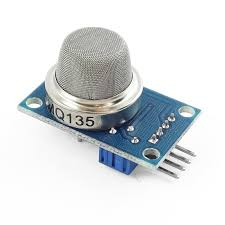
\includegraphics[width=0.3\textwidth]{./mq135}\\[0.1in]
		\label{sensor MQ135}
		\end{figure}
		
		\item \textbf{MQ-7}: It is used to detect Carbon Monoxide in the atmosphere. It is also composed of micro $Al_2O_3$ ceramic tube, Tin Dioxide ($SnO_2$) sensing layer, measuring electrode and heater which are fixed into a crust made by plastic and stainless steel nets. The enveloped MQ-7 has 6 pins, 4 of them are used to fetch signals, and other two are used for providing heating current. Standard measuring circuit of MQ-7, sensing component consist of 2 part, one is heating circuit having time control function (the high voltage and the low voltage work in loop) and the other is the signal output circuit that can accurately respond changes of surface resistance of the sensors.
				\\
				\begin{figure}[h]
				\centering
				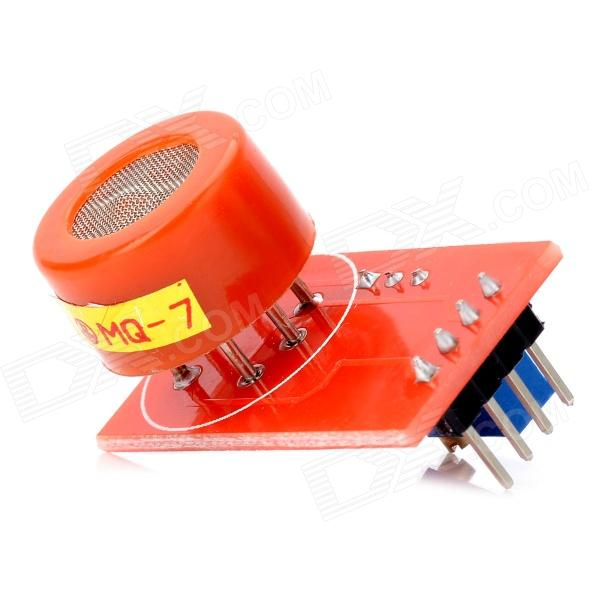
\includegraphics[width=0.3\textwidth]{./mq}\\[0.1in]
				\label{MQ7}
				\end{figure}
		\item \textbf{DHT11}: It features a temperature humidity sensor complexed with calibrated digital signal output. By using the exclusive digital-signal-acquisition technique and temperature humidity sensing technology, it ensures high reliability and excellent long term stability. This sensor includes a resistive type humidity measurement component and an NTC temperature measurement component, and connects to a high performance 8-bit micro-controller, offering excellent quality, fast response, anti-interference ability and also cost-effectiveness.
		\begin{figure}[h]
		\centering
		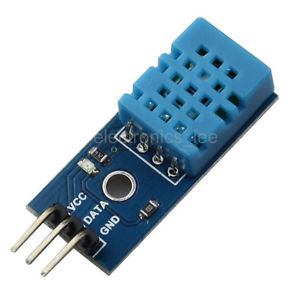
\includegraphics[width=0.3\textwidth]{./DHT11}\\[0.1in]
		\label{DHT11}
		\end{figure}
	\end{itemize}
	
	%\begin{figure}
	%\centering
	%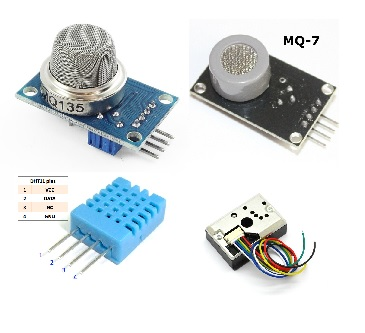
\includegraphics[width=0.8\textwidth]{./sensor}\\[0.1in]
	%\caption{Gas sensors}
	%\label{fig:Gas sensors}
	%\end{figure}

	

	\textbf{Working Principle (Semiconductor Gas Sensor)} : The detection principle of resistive sensors is based on change of the resistance of a thin film upon absorption of the gas molecules on the surface of semi-conductor. The gas-solid interactions affect the resistance of the film because of the density of electronic species in the film. Gas sensor is a subclass of chemical sensors.
\\
\\
Gas sensors measure the concentration of gases in its vicinity. It interacts with a gas to measure it's concentration. Each gas has a unique breakdown voltage i.e. the electric field at which it is ionized. Sensor identifies gas by measuring these voltages. The concentration of the gas can be determined by measuring the current discharge in the device.
\\
\\
	\textbf{Process Flow}:
	\begin{enumerate}
		\item Voltage supply to the sensor.
		\item Ceramic tube made up of $Al_2O_3$ heats up.
		\item Semiconductor chips conductivity is changed due to heating.
		\item Resistance of the circuit changes due to the presence of gas.
		\item Concentration of the gas is calculated by measuring the current since each gas has an unique breakpoint voltage. 
	\end{enumerate}

	\item Optical gas sensors (Dust Sensors) : This type of sensors uses optical absorption/emission scattering of a gas species at defined optical wavelengths. It consists of a light emitting element, a photo detecting element, a gas sensing element responding to light and a filter for picking up fluorescence or phosphorescence. Most optical sensors are usually based on thin films of palladium or chemo chromic oxides coated along the length of an optical fibre. This type of fibre optic sensors are known as optodes. Following methods are used by Optical Sensors\\
	 %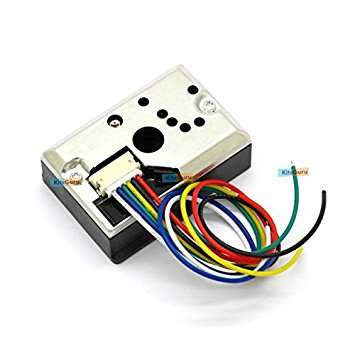
\includegraphics[width=0.8\textwidth]{./dust}\\[0.1in]
	
	\begin{itemize}
		\item Ellipsometry (Technique for the investigation of the dielectric properties)
		\item Spectroscopy (luminescence, phosphorescence, fluorescence, Raman)
		\item Interferometry (white light Interferometry, modal Interferometry in optical waveguide structures)
	\end{itemize}

	In these sensors a desired quantity is determined by:
	\begin{itemize}
		\item Refractive index (speed of light)
		\item Absorbance
		\item Fluorescence properties (of the analyse molecules or a chemo-optical transducing element)
	\end{itemize}

	\textbf{GP2Y1010AU0F} is a dust sensor built on optical sensing system. An infrared emitting diode (IRED) and a phototransistor are diagonally arranged into this device. It detects the reflected light of dust in air. It is effective to detect very fine particle like cigarette smoke.
\begin{figure}
\centering
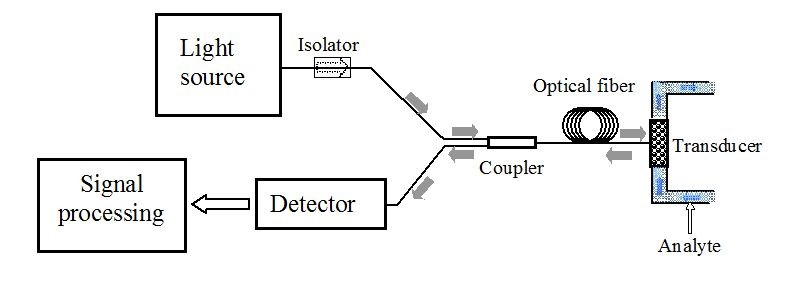
\includegraphics[width=0.8\textwidth]{./optical}\\[0.1in]
\label{fig: Optical sensor}
\caption{Optical sensor}
\end{figure}

	\textbf{Working Principle (Optical Sensors)}:
	\begin{enumerate}
		\item Dust enters through the hole of the sensors.
		\item Infrared emission take place through the IRED.
		\item Reflection of light through dust particles takes place.
		\item As Photo transistor is diagonally arranged to the IRED it gets activated by the refraction. 
		\item The resistance of the Amplifier circuit changes which in turn changes the output voltage.
		\item The concentration of dust is measured by the change in output voltage. 
	\end{enumerate}

\end{enumerate}

\subsubsection{Hight Quality Sensors}
These are the sensors which give stable and more accurate reading with less noise. Following are the Sensors that we have used during our project:

\begin{enumerate}
	\item \textbf{Multichannel Gas Sensor}: It is a built with MiCS-6814 which can detect many unhealthy gases, and three gases can be measured simultaneously due to its three channels, so it can help you to monitor the concentration of more than one gas.  This sensor belongs to Grove System, and you can plug it onto the Grove Base Shield and work with Arduino directly without any jumper wires. It as an I2C interface.

\begin{figure}[h]
	\centering
	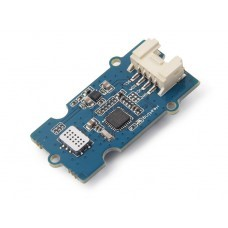
\includegraphics[width=0.4\textwidth]{./multi}\\[0.1in]
	\label{fig:Multichannel gas sensor}
	\caption{Multichannel gas sensor}
	\end{figure}


	\textbf{Detectable Gasses}:
		\begin{itemize}
			\item Carbon monoxide CO (1$-$1000)ppm
			\item Nitrogen dioxide $NO_2$ ( 0.05$-$10 )ppm
			\item Ethanol $C_2H_6$OH (10$–$500)ppm
			\item Hydrogen $H_2$ (1$-$1000)ppm
			\item Ammonia $NH_3$ (1$-$500)ppm
			\item Methane $CH_4$ ($>$1000)ppm
			\item Propane $C_3H_8$ ($>$1000)ppm
			\item Iso-butane $C_4H_{10}$ ($>$1000)ppm
		\end{itemize}
	(Mainly we have used this sensor to measure the concentration of CO and $NO_2$)
	\item Grove – Temperature \& Humidity Sensor (High-Accuracy \& Mini) v1.0: This is a multifunctional sensor that gives you temperature and relative humidity information at the same time. It utilizes a TH02 sensor that can meet measurement needs of general purposes. It provides reliable readings when environment humidity condition in between 0-80\% RH, and temperature condition in between 0-70°C, covering needs in most of the household and daily applications that doesn't reach extreme conditions.
	\\
	\begin{figure}[h]
	\centering
	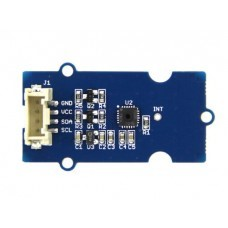
\includegraphics[width=0.4\textwidth]{./temp}\\[0.1in]
	\label{fig:temperature and Humidity sensor}
	\caption{temperature and Humidity sensor}
	\end{figure}
	
	\item PM Dust Sensor Module – Laser Sensing: It is a universal particle concentration measurement digital sensor used to obtain the number of suspended particulate matter in a unit volume of air within 0.3 to 10 microns (concentration of particulate matter) and output with digital interface, also can output quality data of per particle. These sensors can be used in a variety of environmental conditions where it provides timely and accurate concentration data.
\\
\\
	\textbf{Detectable Particulate Matters}: Can detect Particulate Matter of Size 1 Micron, 2.5 Micron and 10 Micron.
\end{enumerate}

\section{Controlling and Processing Unit}

\textbf{A microcontroller} is a small and low-cost microcomputer, which is designed to perform the specific tasks of embedded systems like displaying microwave’s information, receiving remote signals, etc.
\\
\\
\textbf{A microprocessor} is a computer processor which incorporates the functions of a computer's central processing unit (CPU) on a single integrated circuit (IC), [1] or at most a few integrated circuits. [2] The microprocessor is a multipurpose, clock driven, register based, digital-integrated circuit which accepts binary data as input, processes it according to instructions stored in its memory, and provides results as output. Microprocessors contain both combinational logic and sequential digital logic. Microprocessors operate on numbers and symbols represented in the binary numeral system.
\\
\\
\textbf{Difference between Microprocessor \& Microcontroller}:

\begin{center}
 \begin{tabular}{| c |  p{6cm} | p{6cm} |} 
 \hline
 Sl. & Microcontroller & Microprocessor \\ [0.5ex] 
 \hline\hline
 1 & It doesn’t consist of RAM, ROM, I/O ports. It uses its pins to interface to peripheral devices. & It consists of CPU, RAM, ROM, I/O ports. \\ 
 \hline
 2 & Microcontrollers are used to execute a single task within an application. &  Microprocessors are used for big applications. \\
 \hline
 3 & Its designing and hardware cost is low. & Its designing and hardware cost is high. \\
 \hline
 4 & Easy to replace. & Not so easy to replace. \\
 \hline
 5 & It is built with CMOS technology, which requires less power to operate. & Its power consumption is high because it has to control the entire system. \\
 \hline
\end{tabular}
\end{center}

\begin{enumerate}
	\item \textbf{Arduino Mega 2560}: The Mega 2560 is a microcontroller board based on the ATmega2560. It has 54 digital input/output pins (of which 15 can be used as PWM outputs), 16 analog inputs, 4 UARTs (hardware serial ports), a 16 MHz crystal oscillator, a USB connection, a power jack, an ICSP header, and a reset button. It contains everything needed to support the microcontroller; simply connect it to a computer with a USB cable or power it with a AC-to-DC adapter or battery to get started. 

\begin{center}
 \begin{tabular}{| c |  p{6cm} | p{6cm} |} 
 \hline
 Sl. & Microcontroller & Microprocessor \\ [0.5ex] 
 \hline\hline
 1 & Operating Voltage & 5V \\ 
 \hline
 2 & Input Voltage (recommended) & 7-12V \\
 \hline
 3 & Input Voltage (limit) & 6-20V \\
 \hline
 4 & Digital I/O Pins & 54 (of which 15 provide PWM output) \\
 \hline
 5 & Analog Input Pins & 16 \\
 \hline
6 & DC Current per I/O Pin & 20 mA \\
 \hline
7 & DC Current for 3.3V Pin & 50 mA \\
 \hline
8 & Flash Memory Pin & 256 KB of which 8 KB used by bootloader \\
 \hline
9 & SRAM & 8 KB \\
 \hline
10 & EEPROM & 4 KB \\
 \hline
11 & Clock Speed & 16 MHz \\
 \hline
12 & Length & 101.52 mm \\
 \hline
13 & Width & 53.3 mm \\
 \hline
14 & Weight & 37 g \\
 \hline
\end{tabular}
\end{center}

\textbf{Programming}: The Mega 2560 board can be programmed with the Arduino Software (IDE).The ATmega2560 on the Mega 2560 comes pre-programmed with a bootloader that allows you to upload new code to it without the use of an external hardware programmer. It communicates using the original STK500 protocol (reference, C header files).
\begin{figure}
\centering
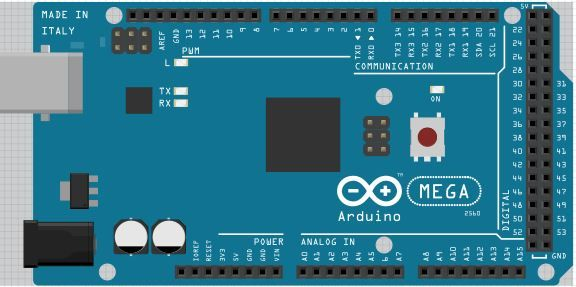
\includegraphics[width=0.6\textwidth]{./arduino}\\[0.1in]
\label{fig:Arduino Mega 2560}
\caption{Arduino Mega 2560}
\end{figure}


\textbf{Warnings}: The Mega 2560 has a resettable poly-fuse that protects your computer's USB ports from shorts and overcurrent. Although most computers provide their own internal protection, the fuse provides an extra layer of protection. If more than 500 mA is applied to the USB port, the fuse will automatically break the connection until the short or overload is removed.
\\
\\
\textbf{Power}: The Mega 2560 can be powered via the USB connection or with an external power supply. The power source is selected automatically. External (non-USB) power can come either from an AC-to-DC adapter (wall-wart) or battery. The adapter can be connected by plugging a 2.1mm centre-positive plug into the board's power jack. Leads from a battery can be inserted in the GND and Vin pin headers of the POWER connector.
\\
\\
The board can operate on an external supply of 6 to 20 volts. If supplied with less than 7V, however, the 5V pin may supply less than five volts and the board may become unstable. If using more than 12V, the voltage regulator may overheat and damage the board. The recommended range is 7 to 12 volts.
\\
\\
\textbf{Memory}: The ATmega2560 has 256 KB of flash memory for storing code (of which 8 KB is used for the bootloader), 8 KB of SRAM and 4 KB of EEPROM.
\\
\\
\textbf{Communication}: The Mega 2560 board has a number of facilities for communicating with a computer, another board, or other microcontrollers. The ATmega2560 provides four hardware UARTs for TTL (5V) serial communication. An ATmega16U2 (ATmega 8U2 on the revision 1 and revision 2 boards) on the board channels one of these over USB and provides a virtual com port to software on the computer (Windows machines will need a .inf file, but OSX and Linux machines will recognize the board as a COM port automatically.
\\
\\
 The Arduino Software (IDE) includes a serial monitor which allows simple textual data to be sent to and from the board. The RX and TX LEDs on the board will flash when data is being transmitted via the ATmega8U2/ATmega16U2 chip and USB connection to the computer (but not for serial communication on pins 0 and 1).

\item \textbf{Raspberry Pi 3 Model B}: 
A Raspberry Pi is a credit card-sized computer originally designed for education, inspired by the 1981 BBC Micro. Creator Eben Upton's goal was to create a low-cost device that would improve programming skills and hardware understanding at the pre-university level. But thanks to its small size and accessible price, it was quickly adopted by tinkerers, makers, and electronics enthusiasts for projects that require more than a basic microcontroller (such as Arduino devices).
\\
\\
The Raspberry Pi is slower than a modern laptop or desktop but is still a complete Linux computer and can provide all the expected abilities that implies, at a low-power consumption level.
\\
\\
The Raspberry Pi is open hardware, with the exception of the primary chip on the Raspberry Pi, the Broadcom SoC (System on a Chip), which runs many of the main components of the board–CPU, graphics, memory, the USB controller, etc. Many of the projects made with a Raspberry Pi are open and well-documented as well and are things you can build and modify yourself.
\\
\\
The Raspberry Pi was designed for the Linux operating system, and many Linux distributions now have a version optimized for the Raspberry Pi. Two of the most popular options are Raspbian, which is based on the Debian operating system, and Pidora, which is based on the Fedora operating system.
\begin{figure}
\centering
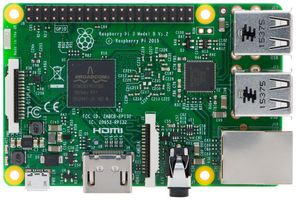
\includegraphics[width=0.6\textwidth]{./pi}\\[0.1in]
\label{fig:Raspberry pi}
\caption{Raspberry pi}
\end{figure}


\textbf{Specification}:
\begin{itemize}
	\item \textbf{SoC}: Broadcom BCM2837 (roughly 50\% faster than the Pi 2)
	\item \textbf{CPU}: 1.2 GHZ quad-core ARM Cortex A53 (ARMv8 Instruction Set)
	\item \textbf{GPU}: Broadcom VideoCore IV @ 400 MHz
	\item \textbf{Memory}: 1 GB LPDDR2-900 SDRAM
	\item \textbf{USB ports}: 4
	\item \textbf{Network}: 10/100 MBPS Ethernet, 802.11n Wireless LAN, Bluetooth 4.0
\end{itemize}

\item \textbf{Additional Component}:
We have used our sensors to gather data and microcontroller (Arduino mega 2560) to control the flow of data but we need to get the real time data of a place and also we need to store the data for data analysis.
\\
\\
\textbf{RTC (Real Time Clock)}: A real-time clock (RTC) is a computer clock (most often in the form of an integrated circuit) that keeps track of the current time. To get the time of a data we have connected RTC with the Arduino mega 2560.
\begin{figure}
\centering
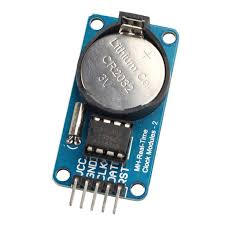
\includegraphics[width=0.3\textwidth]{./rtc}\\[0.1in]
\label{fig: RTC}
\caption{RTC}
\end{figure}

\textbf{SD Card Module and Micro SD card}: SD card module takes the sensor data from the Arduino mega 2560 and store it into the SD card for permanent data storage for further analysis of data. 
\end{enumerate}
%
\includegraphics[width=0.5\textwidth]{./microsd}\\[0.1in]
%\label{Microsd card }




\section{Communication Module}
%VIVEK's PART
\subsection{Architecture}
The data from the Sensors is received by the Arduino Mega 2560 is transferred to the Raspberry Pi(Microprocessor) via serial Communication (Tx and Rx). Data is stored in the memory of Raspberry Pi for further communication. Raspberry Pi is having Bluetooth and WiFi for communication. The Raspberry Pi is Connected to the Internet via Wifi. Data from the raspberry pi send to the firebase database using Firebase API.
Android application is used to fetch the data stored on cloud . Firebase is real time database , Android application fetch the real time data from cloud using Firebase API.Output display the output on the student screen.  

\begin{figure}[!htbp]
	\centering
	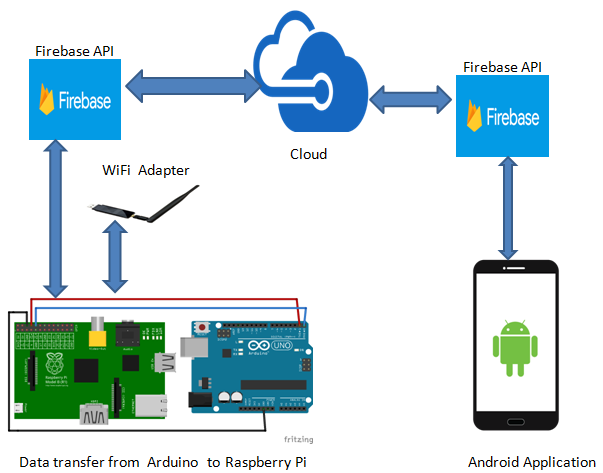
\includegraphics[width=0.9\textwidth]{image1.png}
	\label{fig:Architecture}
	\caption{Architecture}
\end{figure}
 

\subsection{Working of Android Application}

Application needs permission from different hardware, software, internet or any other resource it uses to complete the task. In this application there are four parameter namely Current-Pollution-Status where user can see the current concentration of the pollution of the classroom, Create-Profile where student can create their own profile, view-profile where student can select their profile and compare profile data with the current data of pollutant concentration present in the classroom and Student-Survey in this form student can give their feedback and status of the classroom.
\begin{figure}[!htbp]
	\centering
	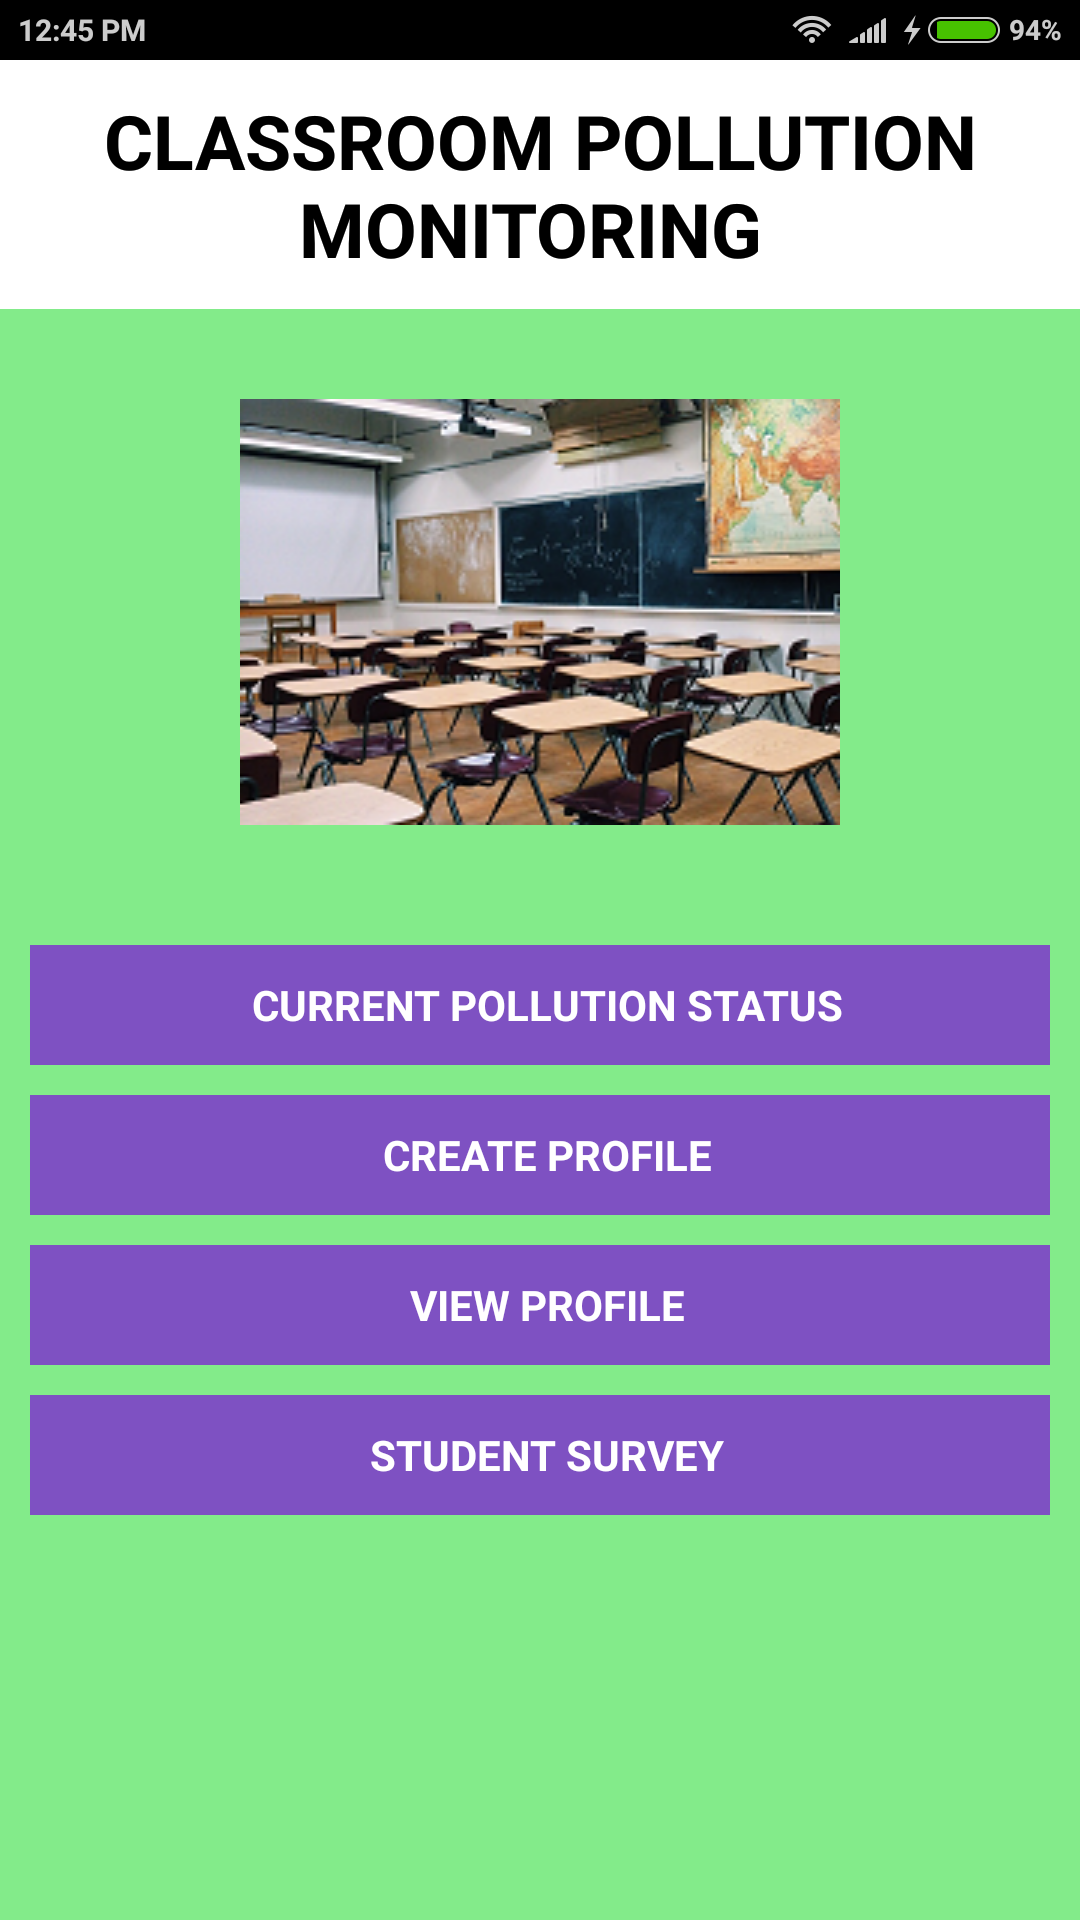
\includegraphics[scale=0.09]{image2.png}
	\label{fig:Working of Android App}
	\caption{Working of Android App}
\end{figure}

\section{Power Module}
The prototype Box can run on AC main power supply current and is also backed up with a 12 V 12 A Battery for load shedding. The Sensors and Microcontrollers require 5 V DC power supply. So we have designed a circuit that will convert the 220 V AC to 5 V DC for smooth running of the device without any power problem.
\\
\\
Also we have installed a 12 V 12 A dry cell battery for power back up.
\\
\\
Sensors and device power used specification.
\\
\\
\begin{center}
 \begin{tabular}{| c |  p{4cm} | p{3cm} | p{3cm} | p{3cm} |} 
\hline
 Sl. & Sensor & Voltage & Current & Power = V * I \\ [0.5ex] 
 \hline\hline
 1 & Arduino Mega 2560 & 5V & 200mA & 1 W \\ 
 \hline
 2 & Laser dust sensor: SKU:SEN0177 & 5V & 200mA & 1 W \\
 \hline
 3 & Temperature and Humidity (TH02) & 5V & 350 micro-A & 1.75 mW \\
 \hline
 4 & Grove - Multichannel gas sensor & 5 V & 30 mA & 150 mW \\
 \hline
 5 & MQ-135 & 5 V & 160 mA & 800 mW \\
 \hline
6 & SD card Module & 5 V & 100 mA & 500mW \\
 \hline
7 & RTC & 5 V & 100 mA & 500 mW \\
 \hline
  &   &   &  \textbf{Total} & 3.95 W(approx 4 W) \\
 \hline
\end{tabular}
\end{center}

\textbf{Formula used}: $$Power = Voltage x Current$$
\\
\\
So we have calculated that our device is drawing approximately 4 W of current.
\\
\\
\textbf{Calculation of Time taken for batter to discharge}:
\\
\\
As we have mentioned that our device is batter enabled for load shedding so we have done a small calculation to find out the duration for the use of batter in case of emergency.
\\
\\
Battery:
\\
\\ 
The specifications of the battery are as follows: 

	$$Voltage = 12 V$$
	$$Current = 12 A$$
	
With the equation to find the power
	$$Power = Voltage x Current$$ \\
		
		$$Total Power of the battery is = (12 x 12) W$$
		$$= 144 W$$
\\
\\
Device:
\\
\\
	
From the above table the total power used by the box  = 4 W
\\
\\
Now we will calculate the time taken for the battery to discharge
$$Time = Battery power / Device power$$\\
	$$= 144 W / 4 W$$
	$$= 36 Hours $$
\\
\\
So our device will run for approximately 36 hours on battery too.

\vspace{0.4in}
\section {Prototype Device}
\vspace{0.2in}
With all these Components combined we have build our prototype device. We named our Device "Environment Monitoring System". The images of our prototype image are given below.
\begin{figure}[!htpb]

\begin{subfigure}
\centering
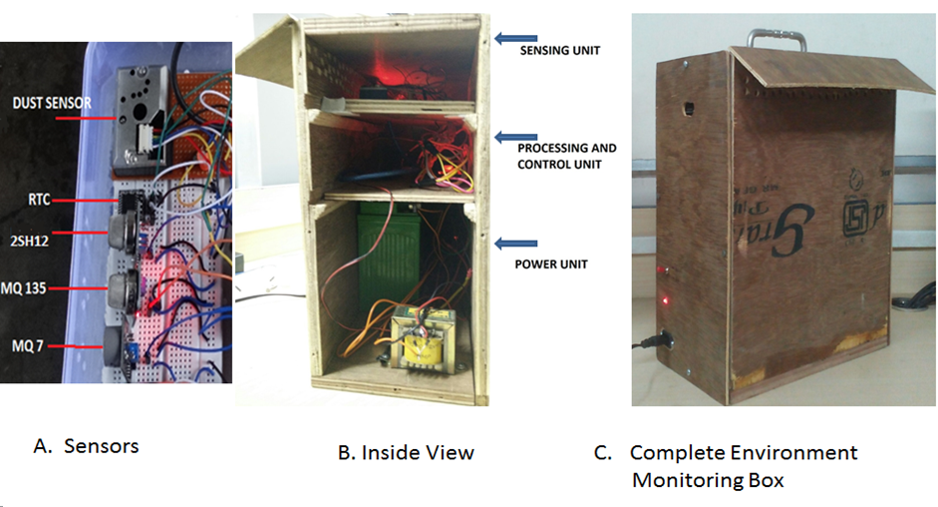
\includegraphics[width=0.8\textwidth]{./prototype_final}\\[0.1in]
\label{fig: Air Quality Monitoring Box}
\caption{AQM Box}
\end{subfigure}

\begin{subfigure}
\centering
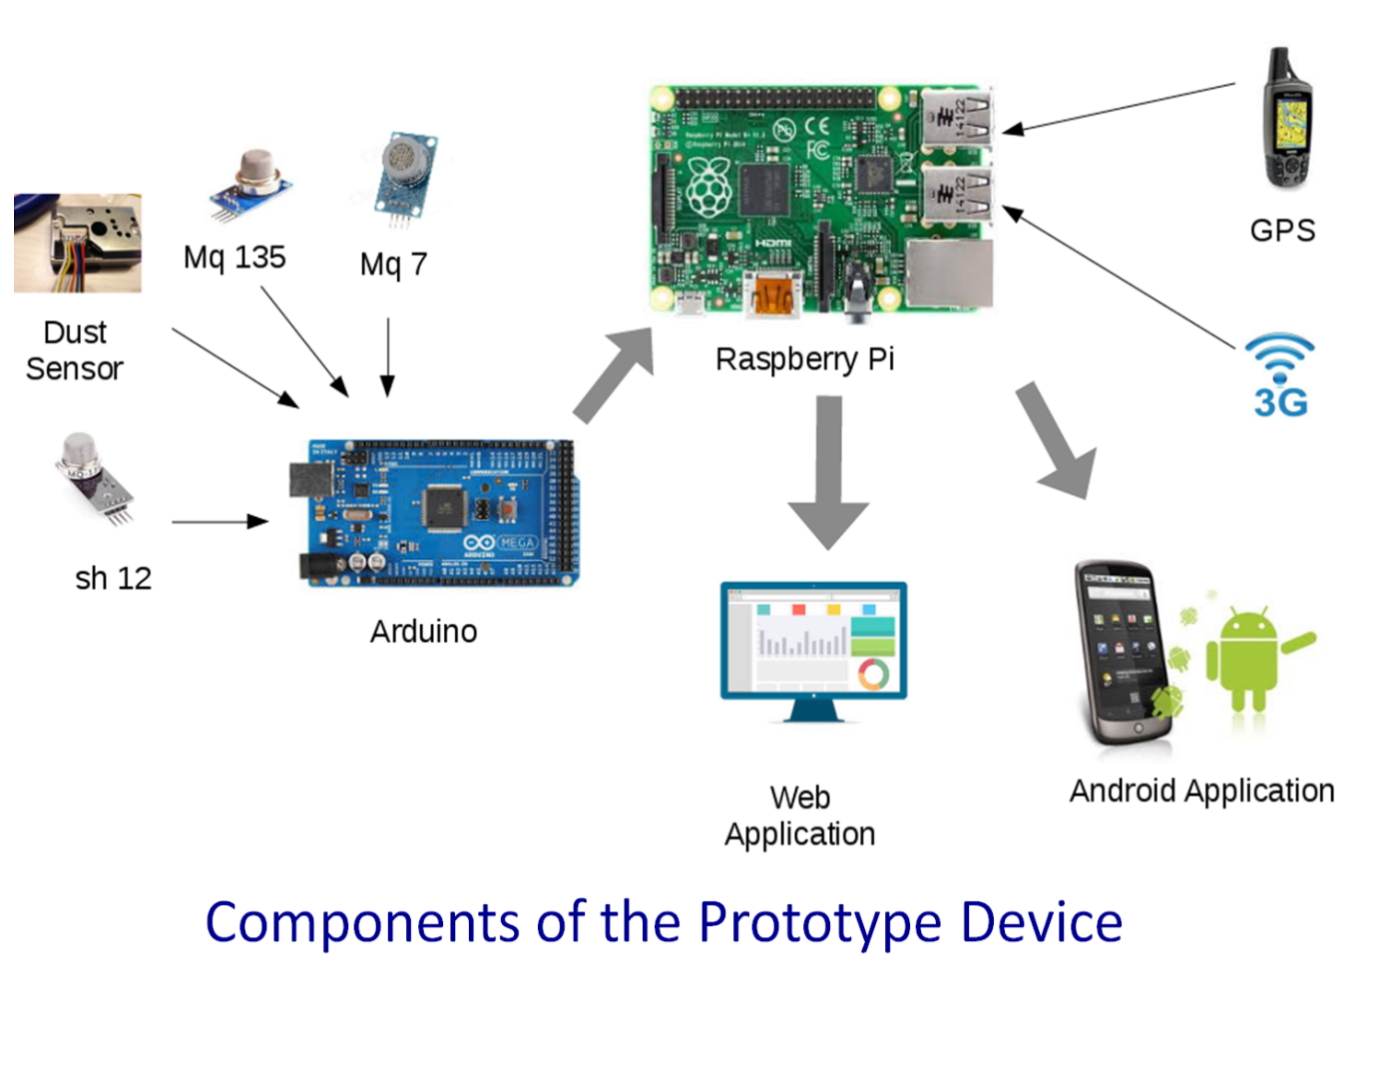
\includegraphics[width=0.8\textwidth]{./prototype_arch}\\[0.1in]
\label{fig: Air Quality Monitoring Box Architecture}
\caption{AQM Box Arch}
\end{subfigure}

\end{figure} %architecture included
\chapter{Data Validation}

\section{WBPCB}

\textbf{West Bengal Pollution Control Board} (WBPCB) keeps tracks of the pollutant data in some of the cities in the state. This is conducted at various monitoring stations in the state and near the polluting clusters of industries. Specific parameters like Oxides of Sulfur, Oxides of Nitrogen, Respirable Particulate Matter etc. are monitored in the ambient air quality monitoring stations. Data of ambient air quality monitoring stations are presented at the web site of the Board (http://www.wbpcb.gov.in/). \\

WBPCB has their monitoring station in our city of Durgapur too. The station is situated Sidhu Kanhu Indoor Stadium, Recol Park, city Centre, Durgapur, West Bengal 713216.(Coordinates : 23°32'25"N   87°17'29"E)

\vspace{0.1in}

\begin{figure}[!htbp]
	\centering
	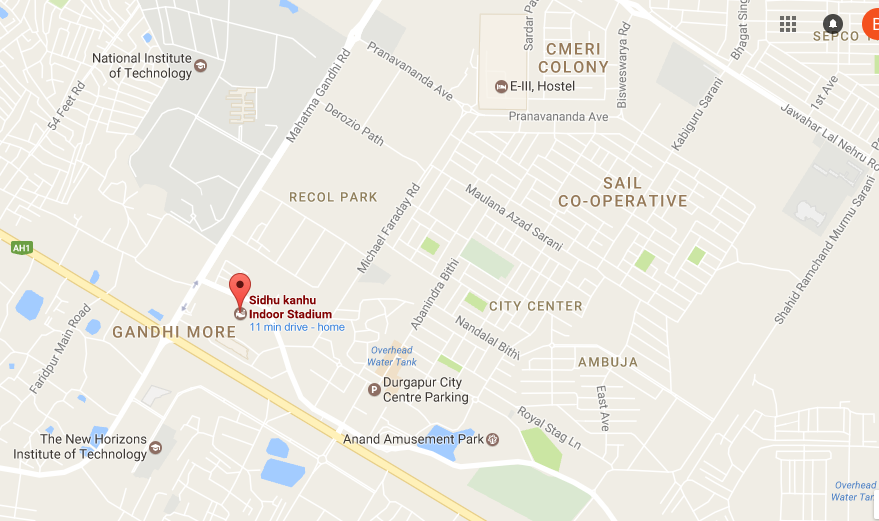
\includegraphics[width=0.7\textwidth]{wbpcb.png}
	\label{fig:Map showing location of WBPCB Stations}
	\caption{Map showing location of WBPCB Stations}
\end{figure}

WBPCB is using sampling based technology to keep track of the pollutants and they upload the hourly data of the area However our Box uses a sensor based technology for the same.\\

\textbf{They are monitoring concentration of pollutants which are Particulate Matter size 10 Micron(PM10), Nitrogen Dioxide (NO2), Sulphur dioxide (SO2), Carbon Monoxide (CO) and Ozone (O3).}.
The pollutants concentration data coming from the Environment Monitoring Box is validated against the WBPCB monitored data to check the efficiency of the data. This process in also called \textbf{Soft Calibration}.

\section{Deployment}

We have deployed our Environment Monitoring Box near to the WBPCB station in Durgapur. The deployment site is 300 m away from the WBPCB station.The box is deployed in the roof top of Pinacle Infotech, Near Junction Mall, City Centre, Durgapur, West Bengal.

\vspace{0.2in}

\begin{figure}[!htbp]
	\centering
	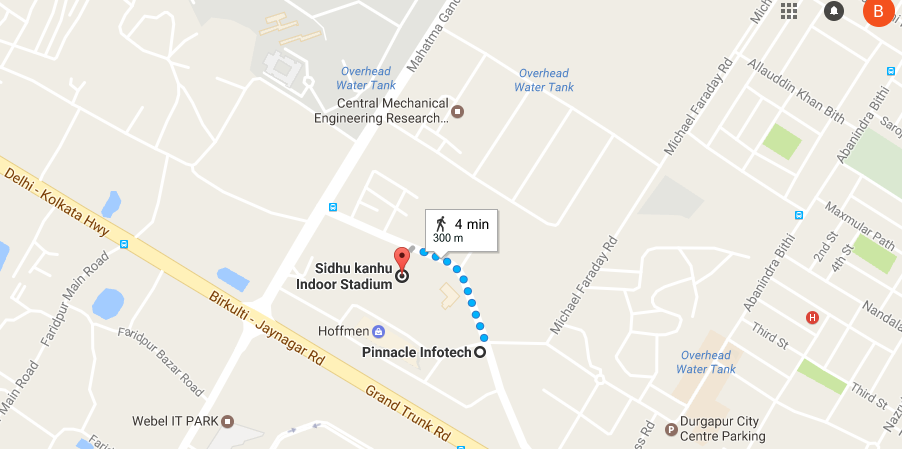
\includegraphics[width=0.9\textwidth]{deployment.png}
	\label{fig:Map showing Our EMB deployment site near to WBPCB station}
	\caption{Map showing Our EMB deployment site near to WBPCB station}
\end{figure}

\vspace{0.1in}
We have taken the reading for 24 hours duration. I.e.17TH May 2017, 12:00 PM to 18TH May 2017, 12:00 PM.

\section{Results and Analysis}
As Mentioned above, the WBPCB station data give the value for (PM10, CO, NO2, SO2), So we have validated the box for (PM10,CO and NO2) only, as we were not having SO2 at the time.
Also The WBPCB station is giving hourly data but our Box is giving data per second so we have calculated mean of the data of the box.
\\
Also we have selected ppm as a unit for measurement of CO and NO2 but WBPCB station gives the data in unit of(mg/m\textasciicircum3) . So we needed to convert.

\subsection{Conversion Formula for ppm(parts per Million) to mg/$m^3$}

mg/$m^3$ = (ppm*molecular weight )/24.45
\\
\\
Here, Molecular weight belongs to individual gases. 

Molecular weight for NO2 is 46.01.

Molecular Weight for CO is 28.01.

\subsection{Plots}
After Collecting the data from WBPCB website for the above said dates and time and from our Box.
The data is labelled as WBPCB for WBPCB station data and BOX for our Box data.

The comparison plots for CO, NO2 and PM10 are:


\begin{figure}[!htbp]
	\centering
	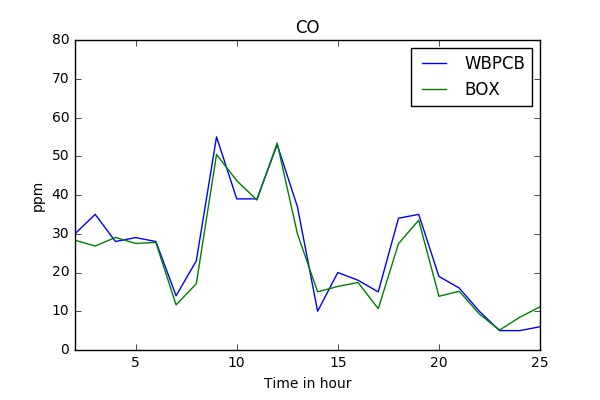
\includegraphics[width=0.9\textwidth]{co.jpg}
	\label{fig:Comparison of CO data}
	\caption{Comparison of CO data}
\end{figure}

\begin{figure}[!htbp]
	\centering
	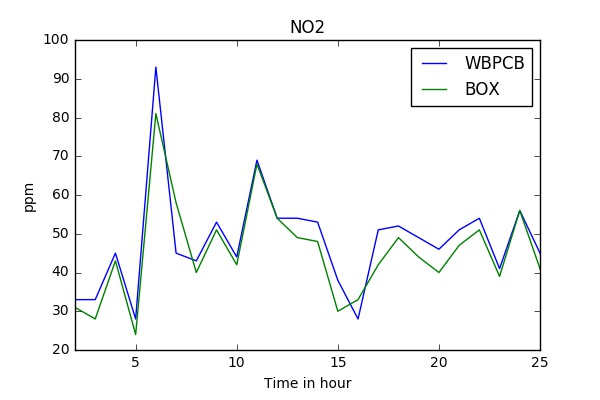
\includegraphics[width=0.9\textwidth]{no2.jpg}
	\label{fig:Comparison of NO2 data}
	\caption{Comparison of NO2 data}
\end{figure}

\begin{figure}[!htbp]
	\centering
	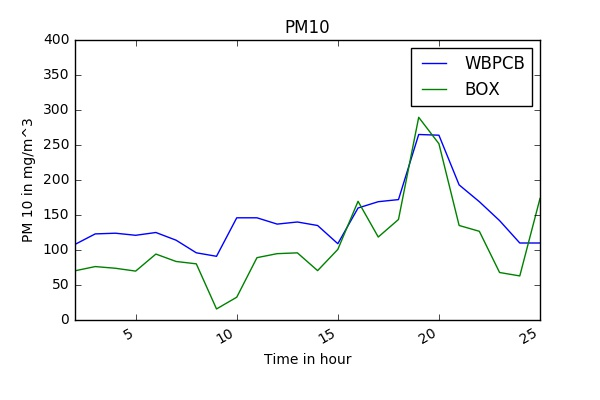
\includegraphics[width=0.9\textwidth]{pm10_compare.jpg}
	\label{fig:Comparison of PM 10 data}
	\caption{Comparison of PM 10 data}
\end{figure}

The Mean difference between the reading of WBPCB station data and our box data is summarized in the following table

\begin{figure}[!htbp]
	\centering
	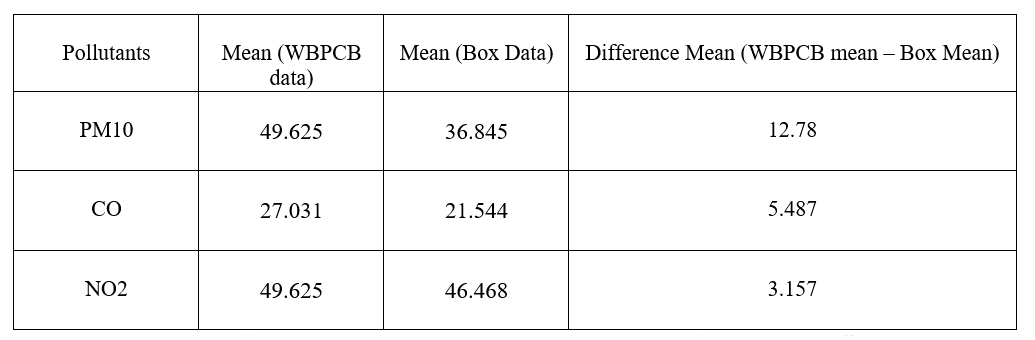
\includegraphics[width=0.9\textwidth]{table.jpg}
	\label{fig:Table showing Mean difference between the Data from WBPCB station and Box data for different pollutants}
	\caption{Table showing Mean difference between the Data from WBPCB station and Box data for different pollutants}
\end{figure}

\newpage
\section{Inferences}

The following conclusion can be drawn from the Plots:

\begin{enumerate}
	\item The Range of our data is same as that of WBPCB for all the three pollutants
	\item Though the value is exactly not same but it is very close to the reading of the WBPCB station (which is high quality sampling based system).
	\item The signature of the curves are same which signifies that our Box is able to catch the variations of data.
\end{enumerate} %result and analysis included
%\chapter{Conclusion}

<Conclusion here>

\cleardoublepage
%\pagebreak
\phantomsection
\addcontentsline{toc}{chapter}{References}
\begin{thebibliography}{99}

\bibitem{citation-1-wikipedia}wikipedia,\ \url{<wikipedia.org/wiki/Pollution>}

\bibitem{citation-2-}Durgapur adda,\ \url{<Durgapuradda.com>}

\bibitem{citation-3-}Tata steel discharge in Kharki river Jamshedpur,\ \url{<Stained steel>}
\bibitem{citation-4-}Durgapur coalmine in chandrapur,\ \url{<wordpress.com>}
\bibitem{citation-5-}Noise within limits,\ \url{google.com}
\bibitem{citation-6-}2 know about,\ \url{google.com}
\bibitem{citation-7-}Mortality linked to air pollution,\ \url{atlas.com}
\bibitem{citation-8-}pollution disasters,\ \url{<www.allianz.com}
\bibitem{citation-9-}Pollution breakpoint,\ \url{<Datadrivenyale.com>}
\bibitem{citation-10-}World Health Organisation,\ \url{who.int}
\bibitem{citation-11-}Greenpeace,\ \url{www.greenpeace.org}
\bibitem{citation-12-}Deadly Air Pollution,\ \url{who.int}
\bibitem{citation-13-}The Economic consequences of Air Pollution,\ \url{<oecd.org>}
\bibitem{citation-14-}Time of India,\ \url{<TimesofIndia.Indiatimes.com>}
\bibitem{citation-15-}Khedo, Kavi K., Rajiv Perseedoss, and Avinash Mungur. \textit{"A wireless sensor network air pollution monitoring system." arXiv preprint arXiv:1005.1737 (2010)}.\ \url{}
%\bibitem{citation-16-}Indoor Air Quality in Homes Offices & Resturants in Korean Urban Areas Indoor Outdoor Relationship\ \url{}
\bibitem{citation-16-}Baek, Sung-Ok, Yoon-Shin Kim, and Roger Perry. "Indoor air quality in homes, offices and restaurants in Korean urban areas—indoor/outdoor relationships.\textit{" Atmospheric Environment 31.4 (1997): 529-544}.
\ \url{}

\bibitem{citation-17-}Lee, Shun Cheng, Wai-Ming Li, and Chio-Hang Ao. "Investigation of indoor air quality at residential homes in Hong Kong—case study.\textit{" Atmospheric Environment 36.2 (2002): 225-237}. 

\bibitem{citation-18-}Jiang, Yifei, et al. "MAQS: a personalized mobile sensing system for indoor air quality monitoring.\textit{" Proceedings of the 13th international conference on Ubiquitous computing ACM, 2011}.\ \url{}
\bibitem{citation-19-}Detecting Indoor Air Pollutants and taking safety measures\ \url{}

\bibitem{citation-20-}Air Sensing and Alert Generation\ \url{}
\bibitem{citation-21-}Environment Monitoring and Air Quality Prediction\ \url{}

\bibitem{citation-22-}Inferring Air Quality and location by using semi-supervised inference model Based on Urban Big Data Technology\ \url{}
\bibitem{citation-23-}Mobile Environment Monitoring\ \url{}

\bibitem{citation-24-}Corani, Giorgio. "Air quality prediction in Milan: feed-forward neural networks, pruned neural networks and lazy learning.\textit{" Ecological Modelling 185.2 (2005): 513-529.}\ \url{}
\bibitem{citation-25-}Al-Ali, A. R., Imran Zualkernan, and Fadi Aloul. "A mobile GPRS-sensors array for air pollution monitoring.\textit{" IEEE Sensors Journal 10.10 (2010): 1666-1671.}\ \url{}
\bibitem{citation-26-}Zheng, Yu, Furui Liu, and Hsun-Ping Hsieh. "U-air: When urban air quality inference meets big data.\textit{" Proceedings of the 19th ACM SIGKDD international conference on Knowledge discovery and data mining. ACM, 2013}.
\bibitem{citation-27-}Air Quality Index(AQI)\ \url{}
\bibitem{citation-28-}Oil and Gas spill\ \url{ http://response.restoration.noaa.gov}
 \bibitem{citation-29-}History Of Pollution\ \url{ https://www.pollutionpollution.com}
 \bibitem{citation-30-}\ \url{ https://www.epa.gov}
 \bibitem{citation-31-}Bibek Poddar, Soumyo Dey et al.On Detecting Acceptable Air Contamination in Classrooms using Low Cost Sensors,\textit{ WACI Workshop, COMSNETS 2017}\\
 

\end{thebibliography}

\end{document}
